%%%%%%%% ICML 2026 EXAMPLE LATEX SUBMISSION FILE %%%%%%%%%%%%%%%%%

\documentclass{article}

\usepackage{microtype}
\usepackage{graphicx}
\usepackage{subcaption}
\usepackage{booktabs}
\usepackage{float}
\usepackage{multirow}

\usepackage{hyperref}
\newcommand{\theHalgorithm}{\arabic{algorithm}}

\usepackage[accepted]{icml2026}

\usepackage{amsmath}
\usepackage{amssymb}
\usepackage{mathtools}
\usepackage{amsthm}
\usepackage[capitalize,noabbrev]{cleveref}

\theoremstyle{plain}
\newtheorem{theorem}{Theorem}[section]
\newtheorem{proposition}[theorem]{Proposition}
\newtheorem{lemma}[theorem]{Lemma}
\newtheorem{corollary}[theorem]{Corollary}
\theoremstyle{definition}
\newtheorem{definition}[theorem]{Definition}
\newtheorem{assumption}[theorem]{Assumption}
\theoremstyle{remark}
\newtheorem{remark}[theorem]{Remark}

\usepackage[textsize=tiny]{todonotes}

\icmltitlerunning{Local Intrinsic Dimensionality of Hidden-State Trajectories}

\begin{document}

\twocolumn[
  \icmltitle{Local Intrinsic Dimensionality of Hidden-State Trajectories: \\
  A Geometric Marker of Correct Reasoning in Qwen3}

  \icmlsetsymbol{equal}{*}

  \begin{icmlauthorlist}
    \icmlauthor{Kaiyuan Huang}{yyy}
    \icmlauthor{Gefei Shen}{yyy}
    \icmlauthor{Qiuyang Feng}{yyy}
  \end{icmlauthorlist}

  \icmlaffiliation{yyy}{Harvard University}

  \icmlcorrespondingauthor{Kaiyuan Huang}{kaiyuanh@mit.edu}
  \icmlcorrespondingauthor{Gefei Shen}{gefeishe@mit.edu}
  \icmlcorrespondingauthor{Qiuyang Feng}{frankfen@mit.edu}

  \icmlkeywords{Machine Learning, ICML}

  \vskip 0.3in
]

\printAffiliationsAndNotice{}

\begin{abstract}
Reasoning-capable language models expose an explicit ``thinking'' phase before producing a final answer, yet the internal geometry of this phase is poorly understood. We probe it with Local Intrinsic Dimensionality (LID) of generated-token hidden states in Qwen3 models from 1.7B to 32B parameters on GSM8K, organising the study as two controls and one main experiment. Two controls validate the probe: LID cleanly separates degenerate repetitive generation from ordinary mathematical generation at every scale, and is essentially unmoved when the GSM8K prompt is padded with irrelevant context or with a deliberately repetitive filler. LID therefore tracks the task being executed, not the surface form of the prompt. In a paired think versus no-think comparison we then report two findings. First, the relative ordering of mean LID across the thinking, think-answer, and no-think-answer segments is \emph{not} stable across model scale: at 1.7B the thinking segment has the lowest mean LID, while at 32B it can be the highest, so no ``thinking is a distinct LID regime'' story survives. Second, when generations are stratified by correctness, a clean signal emerges: at every Qwen3 scale we tested, the thinking trajectories of correct generations have higher mean LID than those of incorrect ones, and the correctness gap inside the thinking phase is several times larger than the corresponding gap in either answer segment. We conclude that LID along the thinking trajectory behaves as a geometric correlate of \emph{successful} reasoning rather than as a fixed signature of the thinking mode.\footnote{Code, configs, and per-experiment artifacts: \url{https://github.com/MyssH/6.8610_Group_Project}.}
\end{abstract}
\section{Introduction}

Recent work on large language models (LLMs) shows that allocating additional computation at inference time can substantially improve performance on multi-step problem solving. One family of methods elicits explicit intermediate reasoning through chain-of-thought prompting, scratchpads, or related prompting strategies; another family studies broader test-time scaling strategies such as sampling, search, selection, and verification \citep{wei2023chainofthoughtpromptingelicitsreasoning,nye2021show,wang2023selfconsistencyimproveschainthought,zhang2025surveytesttimescalinglarge,snell2024scaling}. On GSM8K, chain-of-thought prompting raises PaLM 540B accuracy from $17.9\%$ to $56.9\%$ and GPT-3 175B accuracy from $15.6\%$ to $46.9\%$ \citep{wei2023chainofthoughtpromptingelicitsreasoning}. \emph{Why} intermediate reasoning helps, however, remains incompletely understood. One explanation is that generated reasoning decomposes a problem into easier sub-steps \citep{wei2023chainofthoughtpromptingelicitsreasoning}; another is that longer or multiple inference-time trajectories provide additional opportunities for search, aggregation, or verification \citep{wang2023selfconsistencyimproveschainthought,zhang2025surveytesttimescalinglarge}. A related geometric line of work shows that transformer representations change systematically across depth: intrinsic dimensionality can rise in early layers, contract in intermediate layers, and stabilize or form a shallow second peak in later layers \citep{valeriani2023geometryhiddenrepresentationslarge}. These observations motivate a geometric question about reasoning itself: how does the hidden-state geometry evolve while a model generates a reasoning trajectory?

Much of the intrinsic-dimensionality literature we build on analyzes representations \emph{across transformer depth} for fixed inputs, rather than \emph{along the autoregressive generation trajectory} \citep{valeriani2023geometryhiddenrepresentationslarge,van_Aken_2019}. This distinction matters because explicit reasoning is not a single static representation. Each generated token updates the context, changes the next-token distribution, and may move the model into a different region of activation space. Lens-based methods show that intermediate hidden states contain decodable information about current and future model predictions \citep{belrose2023eliciting,pal2023future}. More directly, recent trajectory-level studies of reasoning examine how hidden-state geometry, token-level uncertainty, and step-specific dynamics relate to final-answer correctness and model commitment during chain-of-thought generation \citep{sun2026llm,zur2025road}. We therefore ask whether the \emph{local} geometry of generated hidden-state trajectories carries information about reasoning outcomes that is not visible from final-answer accuracy alone. We use Local Intrinsic Dimensionality (LID) \citep{NIPS2004_74934548} as the probe.

\paragraph{Research questions.}
We organize the work around three questions. (\textbf{Q1}: validity) Does LID, computed on generated-token hidden states, distinguish ordinary task-oriented generation from clearly degenerate generation? (\textbf{Q2}: robustness) Is LID primarily driven by the task being executed, or can superficial prompt structure such as irrelevant context or repetitive boilerplate push the answer trajectory into a low-LID regime? In particular, since degenerate \emph{output} has low LID in Q1, does degenerate \emph{input} have the same effect on otherwise ordinary GSM8K answer generation? (\textbf{Q3}: reasoning signature) When the same GSM8K problems are run in think and no-think modes on Qwen3 models of different sizes, where does any geometric signal associated with explicit thinking appear?

\paragraph{Contributions.}
Our central empirical finding is that LID inside the thinking phase tracks \emph{whether the model gets the answer right}, while simpler segment-level orderings of thinking versus answering are not stable across model scale.

\begin{itemize}
    \item We instantiate LID as a token-level probe over generated-token hidden states of Qwen3 models (1.7B--32B) and show that it cleanly separates ordinary GSM8K generation from constant, short-cycle, and templatic repetition (Exp.\ A).
    \item Using a control in which the GSM8K prompt is padded with irrelevant context or repetitive filler while the task is held fixed, we show that answer-segment LID is essentially unchanged, even when the prompt itself contains repetitive filler (Exp.\ B). This suggests that the measured LID is tied to the generation task rather than simply to surface prompt form.
    \item In a paired think versus no-think comparison (Exp.\ C), we report two findings. (\textbf{C.1}) The relative ordering of mean LID across the thinking, think-answer, and no-think-answer segments is \emph{not} stable across model scale: paired Wilcoxon tests show that the thinking-minus-answer differences flip sign between 8B and 14B. (\textbf{C.2}) When generations are stratified by correctness, a consistent signal appears: at every Qwen3 scale we tested, the thinking trajectories of correct generations have a positive median LID gap over those of incorrect generations (one-sided Mann--Whitney $U$, $p\leq 0.05$), and the gap is several times larger than the corresponding gap in either answer segment.
\end{itemize}

Taken together, the results support a narrow interpretation: LID along the thinking trajectory should not be read as a fixed signature of the thinking mode, but as a geometric correlate of successful reasoning in the Qwen3 GSM8K setting studied here.

\section{Background and Related Work}

\subsection{Inference-time reasoning and test-time compute}
A large body of work shows that language-model performance on multi-step tasks can improve when additional computation is allocated at inference time. Chain-of-thought prompting, scratchpads, zero-shot chain-of-thought, least-to-most prompting, and tree-of-thought methods encourage models to generate intermediate tokens before committing to an answer \citep{wei2023chainofthoughtpromptingelicitsreasoning,nye2021show,kojima2022large,zhou2023least,yao2023tree}. Other methods improve reliability by using multiple sampled solutions, bootstrapped rationales, verifier or process-supervision signals, or broader test-time scaling strategies \citep{wang2023selfconsistencyimproveschainthought,zelikman2022star,lightman2023lets,zhang2025surveytesttimescalinglarge,snell2024scaling}. These studies establish that inference-time reasoning and additional test-time compute can improve observable task performance. They do not, by themselves, specify what geometric changes occur in the model's hidden states while a reasoning trajectory is being generated. Our work addresses this complementary question by measuring local geometry along generated hidden-state trajectories.

\subsection{Faithfulness and mechanistic accounts of CoT}
A separate line of work studies whether the text of a chain-of-thought explanation should be treated as a faithful account of the computation that produced the answer. Empirical studies of CoT faithfulness show that models can produce explanations that are plausible but incomplete, biased, or causally disconnected from the factors that determine the final output \citep{turpin2023language,lanham2023measuring}. Complementary mechanistic and theoretical analyses investigate how step-by-step reasoning is implemented inside transformer models and how intermediate reasoning tokens can change the effective computation available to the model \citep{dutta2024thinkstepbystepmechanisticunderstanding,merrill2023expressive}. Together, these results caution against identifying the visible CoT string with the model's internal computation. This motivates analyses that look beyond the generated text itself. In this paper, we use hidden-state trajectories as the object of study and ask whether their local geometry carries information about successful reasoning.

\subsection{Representation geometry and intrinsic dimensionality}
Representation-level work has shown that transformer activations encode information that varies across layers, including linguistic, syntactic, semantic, and task-relevant structure \citep{van_Aken_2019,ethayarajh2019contextual,tenney2019bert,hewitt2019structural,clark2019bert}. A related geometric literature studies properties such as anisotropy, manifold structure, and intrinsic dimensionality in learned representations. Intrinsic-dimensionality analyses suggest that neural representations often occupy structured subsets of their ambient activation spaces, and that this structure can vary across layers, architectures, and tasks \citep{valeriani2023geometryhiddenrepresentationslarge,ansui2019intrinsic,facco2017estimating}. We build on this literature using the nearest-neighbor maximum-likelihood estimator of intrinsic dimension introduced by \citet{NIPS2004_74934548}, together with later work on Local Intrinsic Dimensionality (LID) estimation and interpretation \citep{amsaleg2015estimating,houle2017local}. LID has also been used to characterize neural activations in settings such as adversarial examples and learned representation geometry \citep{ma2018characterizing,ansui2019intrinsic}. Our contribution is to move from primarily layerwise or dataset-level representation geometry to token-level local geometry along autoregressive generation trajectories.

\subsection{Trajectory-level reasoning signals}
Recent work has begun to analyze language-model computation as an evolving trajectory rather than a single static hidden state. Logit-lens and tuned-lens methods decode intermediate hidden states to study how model predictions become accessible across depth \citep{belrose2023eliciting}. Future Lens similarly asks what future tokens can be anticipated from a single hidden state, providing evidence that intermediate representations contain information about likely continuations \citep{pal2023future}. More directly related to reasoning, recent trajectory-level studies examine how step-specific hidden-state geometry, token-level uncertainty, and hidden-state dynamics relate to reasoning behavior and final-answer correctness \citep{sun2026llm,zur2025road}. These works motivate treating the generation process itself as an object of analysis.

Our study differs from prior trajectory-level work in four respects. First, we compute LID at the token level along generated hidden-state trajectories, rather than relying only on layerwise summaries or final-answer behavior. Second, we use Qwen3's paired think and no-think modes to compare explicit reasoning and direct answering within the same model family, tokenizer, task, and answer format. Third, we stratify trajectories by final-answer correctness, which allows us to distinguish geometry associated with successful reasoning from geometry associated merely with producing a thinking trace. Fourth, we include two controls: degenerate-generation controls showing that LID detects collapsed repetitive output, and prompt-structure controls showing that irrelevant or repetitive prompt padding does not by itself drive the answer trajectory into the same low-LID regime. These design choices support a narrower interpretation of our findings: thinking-phase LID is not a universal signature of CoT text, but a geometric correlate of successful reasoning in the Qwen3 GSM8K setting we study.

\section{Method}
\label{sec:method}

\paragraph{Setup.} For each model, prompt, and generation mode we record the hidden state of every generated token at selected transformer layers $\ell \in \{6, 13, 20\}$. The body reports layer $13$ as a representative intermediate layer; results for layers~$6$ and~$20$ are in Appendix~\ref{app:layer-figures}. We write
\[
H^{(\ell)} = \{h^{(\ell)}_1, h^{(\ell)}_2, \ldots, h^{(\ell)}_n\}, \quad h^{(\ell)}_i \in \mathbb{R}^{d_\ell},
\]
for the sequence of hidden states of a generated \emph{segment} at layer $\ell$. Depending on the experiment, a segment is either a full no-think generation, the thinking sub-segment of a think-mode generation, or the post-thinking answer sub-segment.

\paragraph{Token-level LID.} For a hidden state $h_i^{(\ell)}$ we compute Euclidean distances to all other hidden states in the same segment and sort them: $r_1(h_i^{(\ell)}) \leq \cdots \leq r_k(h_i^{(\ell)})$, where $r_j(h_i^{(\ell)})$ is the distance to the $j$-th nearest neighbor. The Levina--Bickel maximum-likelihood estimator \citep{NIPS2004_74934548} is
\begin{equation}
\widehat{\mathrm{LID}}_k(h_i^{(\ell)}) =
\left(
\frac{1}{k-1}
\sum_{j=1}^{k-1}
\log \frac{r_k(h_i^{(\ell)})}{r_j(h_i^{(\ell)})}
\right)^{-1}.
\label{eq:lid}
\end{equation}
Lower LID indicates that nearby hidden states lie in a more locally constrained region; higher LID indicates a more locally complex neighborhood. We use $k=10$, raw Euclidean distances (no normalization), and aggregate to a segment-level statistic by taking the mean over valid tokens. Segments shorter than $k$ plus a small margin are excluded. Implementation details (sampling parameters, segmentation, accelerator) are in Appendix~\ref{app:implementation}.

\section{Experimental Setup}
\label{sec:setup}

All experiments run on Qwen3 models, which expose both a think and a no-think generation mode while keeping the family, tokenizer, and chat template fixed. We use GSM8K \citep{cobbe2021trainingverifierssolvemath} as the underlying task --- grade-school math word problems with verifiable numeric answers. To make think and no-think answer segments comparable, we use a structured visible-answer format (one-line \texttt{Summary}, one \texttt{Equation}, one \texttt{Final answer}); this prevents no-think generations from collapsing to a single token and keeps the visible answer length comparable across modes. The full template and prompt variants are in Appendix~\ref{app:prompts}.

The evaluation is designed as two controls and one main experiment. Exp.\ A (\cref{sec:exp-a}) tests whether LID is sensitive enough to distinguish degenerate from ordinary generation; without this no downstream comparison is meaningful. Exp.\ B (\cref{sec:exp-b}) tests whether LID survives superficial prompt-structure changes; if surface form drives LID, later think vs.\ no-think differences would be hard to interpret. Exp.\ C (\cref{sec:exp-c}) then runs the paired think vs.\ no-think comparison and asks where the geometric signature of explicit reasoning actually lives.

\section{Experiment A: Validity Test}
\label{sec:exp-a}

Before using LID as a probe of reasoning we ask whether it can at all distinguish ordinary task-oriented generation from clearly low-complexity generation. We hold the model in no-think mode and compare four prompt families: \emph{regular GSM8K} canonical prompts, \emph{constant repetition} (output a single token many times), \emph{short-cycle repetition} (a short cycle repeated many times), and \emph{templatic repetition} (a fixed answer-shaped string repeated many times). The repetition prompts elicit generations whose hidden-state trajectory is forced to revisit a narrow region of activation space.

\begin{figure*}[t]
    \centering
    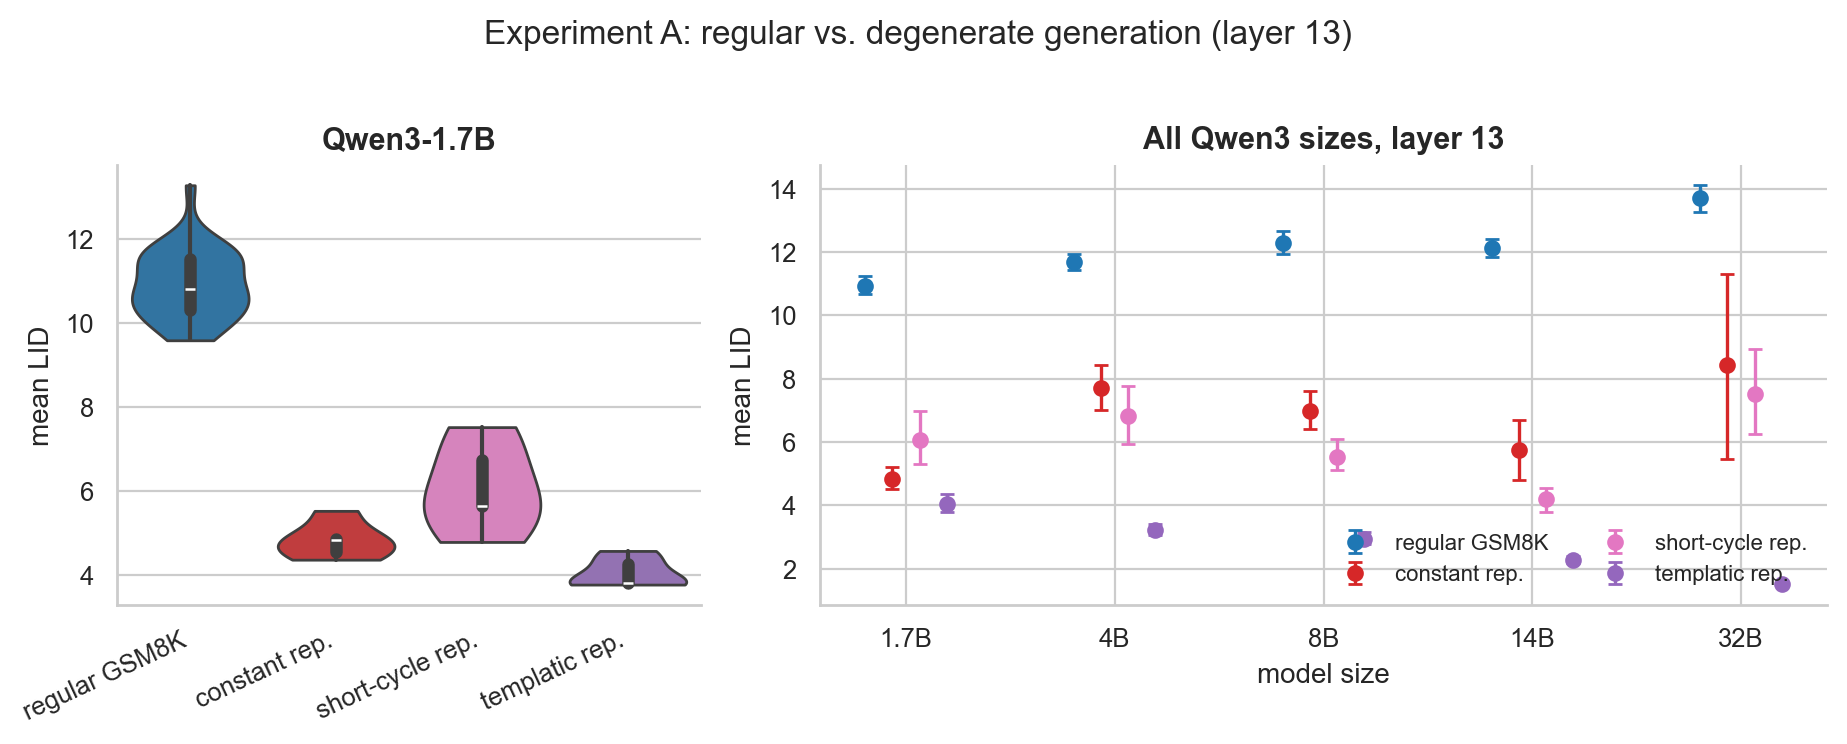
\includegraphics[width=0.95\linewidth]{Images/fig_exp_a_layer13.png}
    \caption{Experiment~A at layer~13. \textbf{Left:} Qwen3-1.7B mean LID by prompt family. \textbf{Right:} mean LID with bootstrap $95\%$ CIs across all Qwen3 scales. Regular GSM8K sits well above all three degenerate families at every scale, with templatic repetition the lowest-LID family.}
    \label{fig:exp-a}
\end{figure*}

\cref{fig:exp-a} (left) shows the layer-13 mean LID for Qwen3-1.7B by family: regular GSM8K generations sit substantially above all three degenerate families with little distributional overlap, and templatic repetition is the lowest of the three, consistent with its rigid output structure. The right panel confirms that the separation is not an artifact of any single scale: regular GSM8K is well above the degenerate families at 1.7B, 4B, 8B, 14B, and 32B; the same pattern holds at layers~6 and~20 (\cref{app:layer-figures}). LID is therefore a usable probe in the sense that it reliably detects when the trajectory collapses into a narrow region. We do not treat this as evidence that ``low LID is bad reasoning'' --- templatic repetition is low-LID but is doing no reasoning at all --- so for now we read LID as a direction-sensitive geometric statistic, not a quality metric.

\section{Experiment B: Robustness Control}
\label{sec:exp-b}

Experiment~A leaves a confound. Repetitive \emph{output} has low LID; does repetitive \emph{input} likewise depress the LID of the model's answer trajectory? If it does, any later think vs.\ no-think comparison risks measuring prompt repetitiveness rather than reasoning. Experiment~B is a no-think-only control designed to rule this out. We keep the GSM8K task and the visible-answer format fixed and vary only the prompt structure across three conditions: \emph{canonical} GSM8K; \emph{irrelevant context} (prepend an unrelated background paragraph); \emph{repetitive filler} (prepend a fixed repeated boilerplate string, see \cref{app:prompts}). The repetitive-filler condition is the key one: its prompt itself contains the same kind of repetition that Experiment~A showed to be associated with very low output LID. If LID is driven by surface form, that repetition should leak into the answer segment.

\begin{figure*}[t]
    \centering
    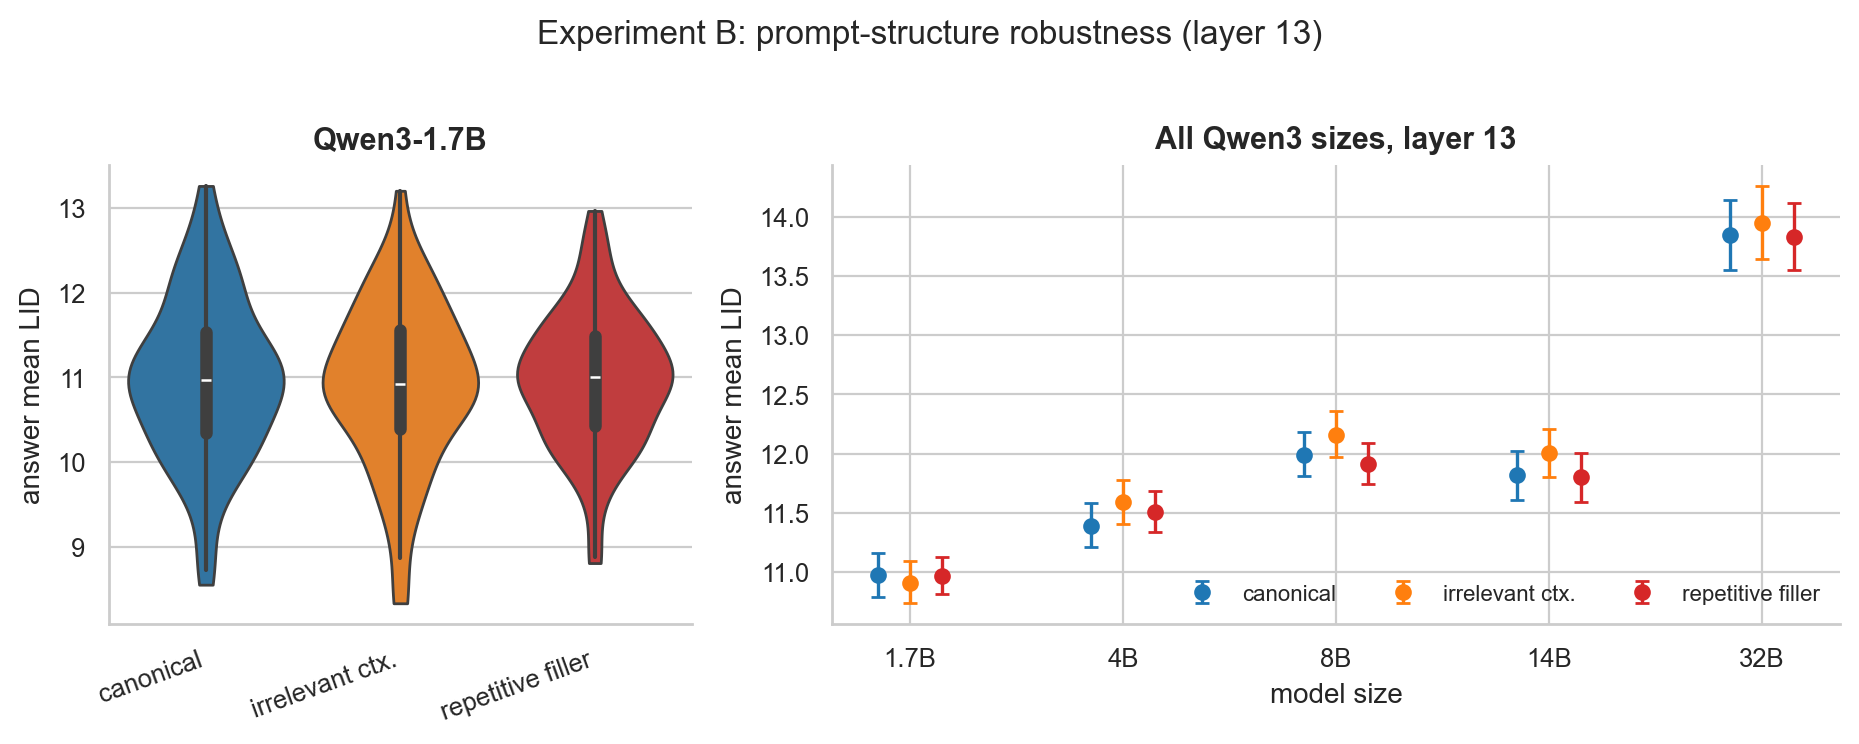
\includegraphics[width=0.95\linewidth]{Images/fig_exp_b_layer13.png}
    \caption{Experiment~B at layer~13. \textbf{Left:} answer-segment mean LID distributions on Qwen3-1.7B for the canonical, irrelevant-context, and repetitive-filler prompts. \textbf{Right:} bootstrap means and $95\%$ CIs across all Qwen3 scales. Within each model the three prompt conditions fall within a small fraction of an LID unit of each other; the dominant axis of variation is model scale, not prompt structure.}
    \label{fig:exp-b}
\end{figure*}

\cref{fig:exp-b} (left) shows the answer-segment LID distributions for Qwen3-1.7B at layer~13: the three conditions are highly overlapping with very similar medians, in clear contrast to the wide separation seen in Experiment~A. The right panel shows that this is true across scales --- within each model the three prompt conditions fall within a small fraction of an LID unit of each other, while the dominant axis of variation is model size. The repetitive-filler prompt, even though it is itself repetitive, does not pull the answer-segment LID toward the degenerate regime. Combined with Experiment~A, this means LID is associated with the \emph{nature of the task being executed}: when the task is degenerate output, LID is low; when the task is regular GSM8K solving, LID is regular, regardless of whether the prompt has been padded with irrelevant or repetitive material.

\section{Experiment C: Think vs.\ No-Think Reasoning}
\label{sec:exp-c}

Experiment~C is the main comparison between explicit thinking and direct answering. For each GSM8K problem we run the model twice, once in think mode and once in no-think mode. In think mode the output is split into a \emph{thinking segment} (the explicit reasoning block) and a \emph{think-answer segment} (the final answer produced after thinking); in no-think mode we analyse the \emph{no-think-answer segment} directly. The result is three phases per pair: \texttt{thinking}, \texttt{think\_answer}, and \texttt{no\_think\_answer}. We report two findings. C.1 is a negative result at the level of segment means; C.2, the main finding, appears only after conditioning on whether the model got the answer right.

\subsection{C.1: Segment ordering is not stable across scale}
\label{sec:exp-c-segment}

A natural first hypothesis is that explicit thinking sits in a distinctive LID regime relative to direct answering --- either consistently \emph{lower} (a more rigid ``reasoning manifold'') or consistently \emph{higher} (a more exploratory phase). Our data do not support either reading.

\begin{figure*}[t]
    \centering
    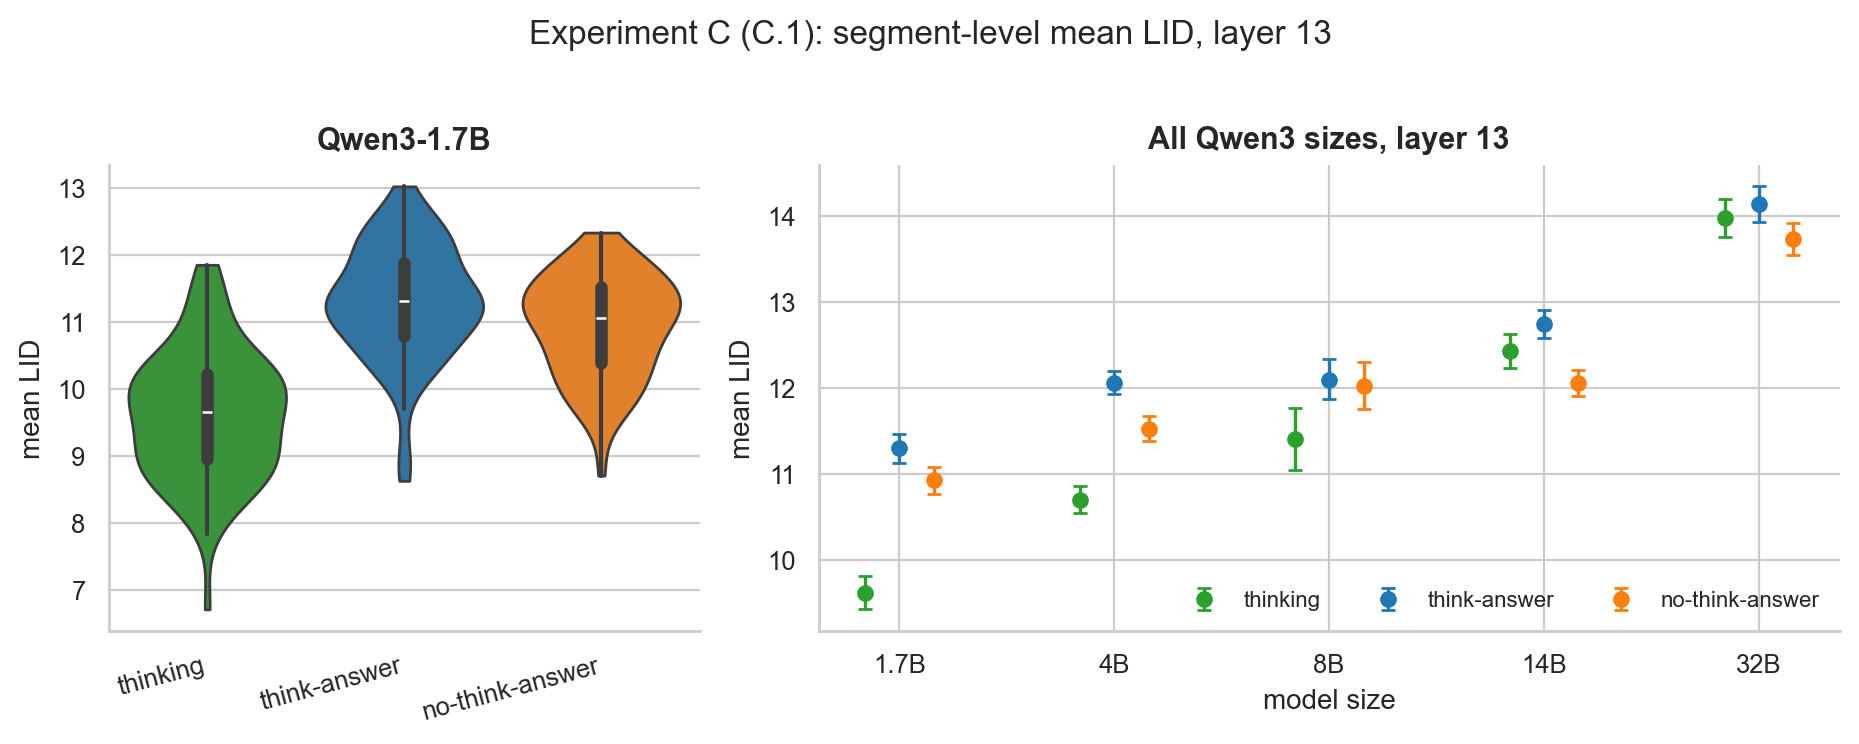
\includegraphics[width=0.95\linewidth]{Images/fig_exp_c_segments_layer13.png}
    \caption{Experiment~C, C.1 at layer~13. \textbf{Left:} per-segment mean LID for Qwen3-1.7B (thinking is the lowest-LID phase). \textbf{Right:} bootstrap means and $95\%$ CIs of the three segments across Qwen3 scales. The thinking segment is at the \emph{bottom} of the three at 1.7B and 4B but moves to the \emph{top} at 32B, so segment ordering is not scale-invariant.}
    \label{fig:exp-c-segment}
\end{figure*}

\cref{fig:exp-c-segment} (left) shows that at Qwen3-1.7B the thinking segment is the lowest-LID phase, with the two answer segments visibly above it, which superficially supports the ``thinking is structurally simpler'' reading. The right panel shows that this ordering does not hold across model sizes: at 1.7B and 4B the thinking segment is at or near the bottom of the three segments at layer~13; at 14B and 32B it is comparable to or above the answer segments; and the orderings at layers~6 and~20 shift again (\cref{app:layer-figures}). Layer-13 mean LIDs from our runs make the magnitude concrete: at 1.7B, thinking is $9.62$ vs.\ think-answer $11.30$ vs.\ no-think-answer $10.93$; at 32B, the three values are $13.98$, $14.14$, and $13.74$ respectively --- almost identical, with the thinking segment now at the \emph{top}.

\begin{table}[t]
    \centering
    \footnotesize
    \begin{tabular}{lrrr}
    \toprule
    Model & thinking $-$ & thinking $-$ & think\_ans $-$ \\
          & think\_ans   & no\_think\_ans & no\_think\_ans \\
    \midrule
    1.7B & $-1.72^{\star\star\star}$ & $-1.20^{\star\star\star}$ & $+0.43^{\star\star\star}$ \\
    4B   & $-1.39^{\star\star\star}$ & $-0.67^{\star\star\star}$ & $+0.48^{\star\star\star}$ \\
    8B   & $-0.49^{\star\star\star}$ & $-0.50^{\star}$           & $+0.26$ \\
    14B  & $-0.08^{\star}$           & $+0.40^{\star\star\star}$ & $+0.59^{\star\star\star}$ \\
    32B  & $+0.05$                   & $+0.40^{\star}$           & $+0.36^{\star\star\star}$ \\
    \bottomrule
    \end{tabular}
    \caption{C.1, layer~13. Paired Wilcoxon signed-rank tests on segment-wise differences of mean LID, per model. Entries are median paired differences. Significance: $\star\,p<0.05$, $\star\star\,p<0.01$, $\star\star\star\,p<10^{-3}$ (two-sided). The thinking $-$ answer differences \emph{flip sign} between 8B and 14B; no global segment ordering is stable across scale. Full $p$-values, counts, and layers $6$ and $20$ are in Appendix~\ref{app:wilcoxon-tables}.}
    \label{tab:c1-wilcoxon-layer13}
\end{table}

To make the lack of a stable ordering precise we run, for each model and at layer~13, a paired Wilcoxon signed-rank test on segment-wise differences, joining the thinking and answer segments by GSM8K example~ID (\cref{tab:c1-wilcoxon-layer13}). The thinking $-$ answer differences are large and strongly negative at 1.7B and 4B ($p\!<\!10^{-12}$ in both pairings), are smaller but still negative at 8B, and \emph{flip sign} at 14B and 32B, where the thinking median is at or above both answer medians. The think-answer $-$ no-think-answer difference, by contrast, is positive at every scale but its magnitude is small and at 8B is not significant. Layers $6$ and $20$ (Appendix~\cref{tab:c1-wilcoxon-full}) show the same picture with a different specific tilt: at layer~6 the sign flip is even more extreme (thinking is the lowest segment at 1.7B but the highest at 32B); layer~20 is genuinely model-dependent.

The negative takeaway is that segment-level mean LID is not, by itself, a stable signature of the thinking mode. Whatever geometric correlate of reasoning we are looking for, it is not just ``thinking sits in a different LID regime from answering''.

\subsection{C.2: Correct generations have higher thinking LID --- across all model sizes}
\label{sec:exp-c-correctness}

When we stratify the same paired generations by whether the final answer is correct, a consistent signal appears inside the thinking phase. \cref{fig:exp-c-correctness} shows mean LID per phase, split by correctness, with each model and each of the three phases as a separate sub-panel. In the leftmost panel (\texttt{thinking}), the green ``correct'' point sits above the red ``wrong'' point at \emph{every} Qwen3 scale; in the middle and rightmost panels (\texttt{think-answer} and \texttt{no-think-answer}) the two points overlap, with no consistent direction. \cref{fig:exp-c-correctness-gap} summarises this in one chart by plotting the median correct-minus-wrong LID gap per phase per model: the thinking-phase gap (green) is consistently positive and substantially larger than the gaps in either answer phase (blue/orange), which are close to zero and inconsistent in sign. Averaged across the layers we instrument, the correct-minus-incorrect mean-LID gap is approximately $0.30$ in the no-think-answer segment, $0.44$ in the think-answer segment, and $3.11$ in the thinking segment --- an order-of-magnitude separation in favour of the thinking phase.

\begin{figure*}[t]
    \centering
    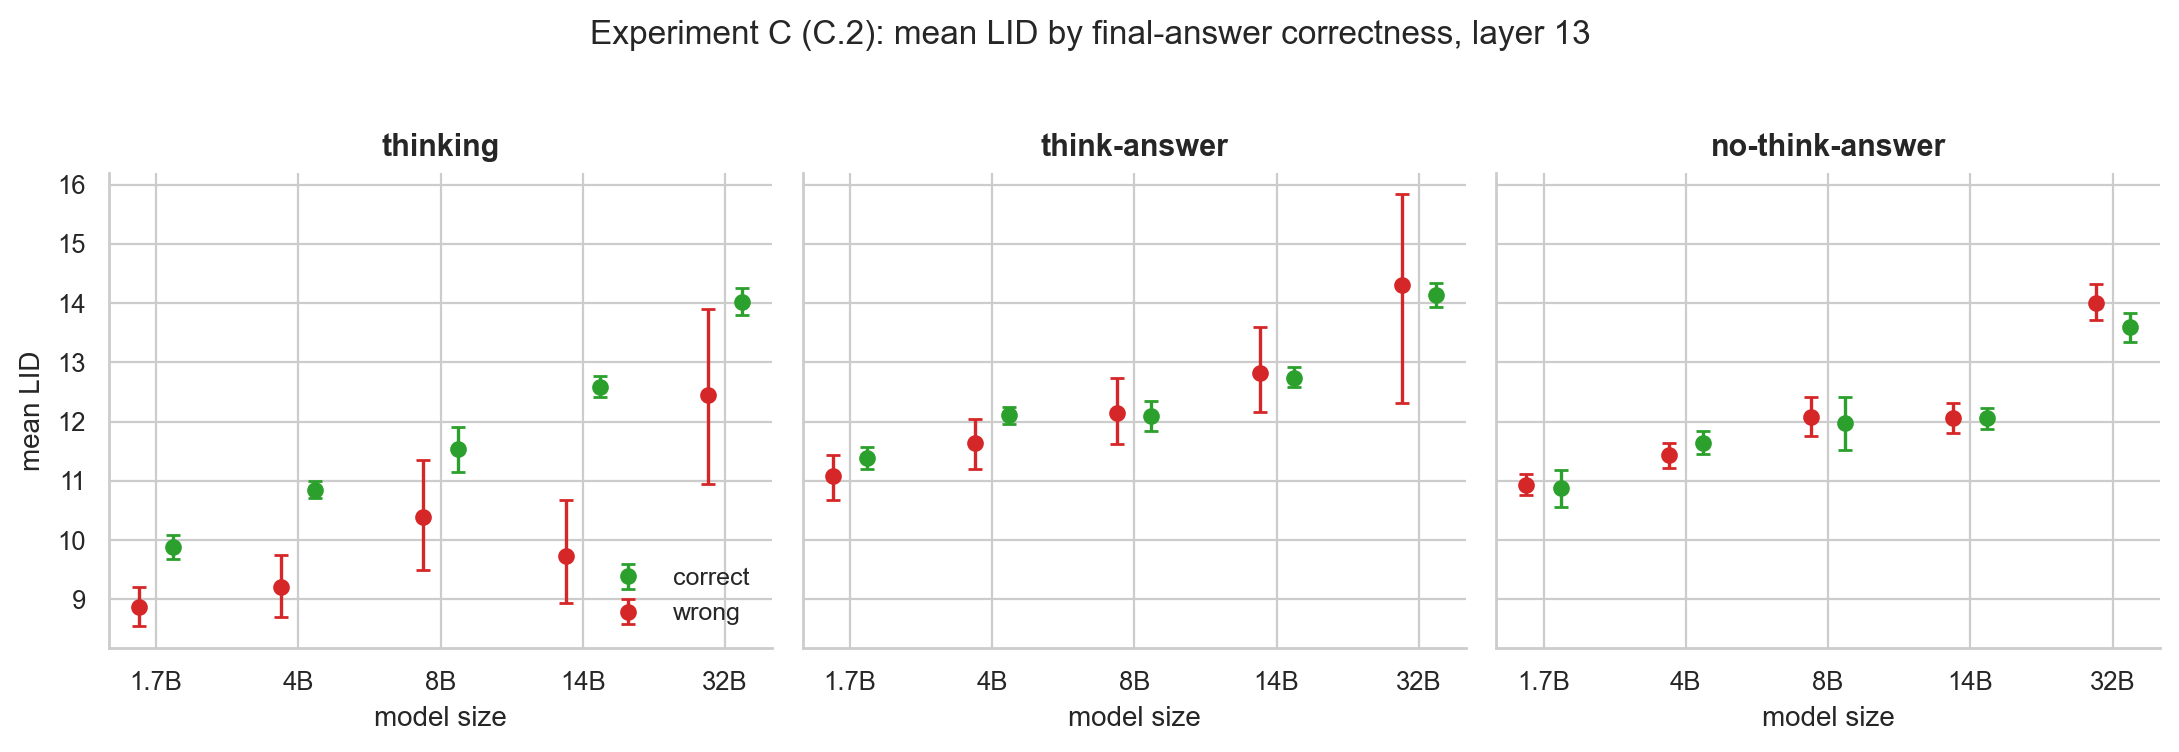
\includegraphics[width=0.95\linewidth]{Images/fig_exp_c_correctness_layer13.png}
    \caption{Experiment~C, C.2 at layer~13: mean LID by final-answer correctness, plotted per phase. Green: correct; red: wrong. Error bars are bootstrap $95\%$ CIs. In the thinking phase (left), the correct point sits above the wrong point at every Qwen3 scale; in the two answer phases (middle, right), the two points overlap with no consistent direction.}
    \label{fig:exp-c-correctness}
\end{figure*}

\begin{figure}[t]
    \centering
    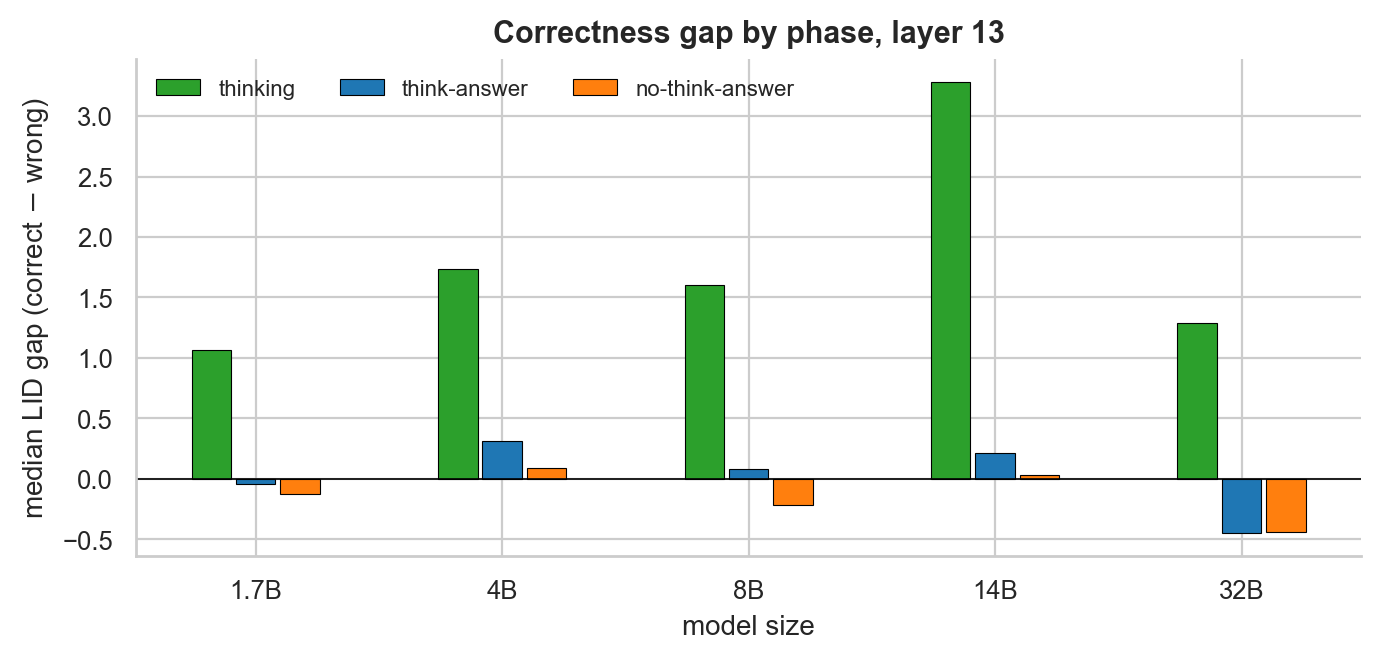
\includegraphics[width=\columnwidth]{Images/fig_exp_c_correctness_gap.png}
    \caption{C.2 headline summary at layer~13. Median LID gap (correct $-$ wrong) per phase per model. The thinking-phase gap (green) is positive at every scale and an order of magnitude larger than the think-answer (blue) and no-think-answer (orange) gaps, which are close to zero and inconsistent in sign.}
    \label{fig:exp-c-correctness-gap}
\end{figure}

\begin{table}[t]
    \centering
    \footnotesize
    \begin{tabular}{lrrrrr}
    \toprule
    Model & $n_{\text{c}}$ & $n_{\text{w}}$ & $\widetilde{\text{LID}}_{\text{c}}$ & $\widetilde{\text{LID}}_{\text{w}}$ & gap, $p$ \\
    \midrule
    1.7B & $67$  & $23$ & $9.86$  & $8.79$  & $+1.06^{\star\star\star}$ \\
    4B   & $182$ & $18$ & $10.87$ & $9.13$  & $+1.74^{\star\star\star}$ \\
    8B   & $55$  & $7$  & $11.63$ & $10.02$ & $+1.61^{\star}$ \\
    14B  & $189$ & $11$ & $12.58$ & $9.30$  & $+3.29^{\star\star\star}$ \\
    32B  & $194$ & $6$  & $14.00$ & $12.71$ & $+1.29^{\star}$ \\
    \bottomrule
    \end{tabular}
    \caption{C.2, layer~13. One-sided Mann--Whitney $U$ tests of correct vs.\ incorrect thinking-phase mean LID, per model. $n_{\text{c}}$, $n_{\text{w}}$: counts of correct / incorrect think-mode pairs; $\widetilde{\text{LID}}$: median mean LID. Significance: $\star\,p<0.05$, $\star\star\,p<0.01$, $\star\star\star\,p<10^{-3}$. \textbf{Every model shows a positive gap and rejects at $p\!\leq\!0.05$.} Full per-phase tables and layers $6$ and $20$ are in Appendix~\ref{app:wilcoxon-tables}.}
    \label{tab:c2-wilcoxon-layer13}
\end{table}

We make the per-model statement precise with a one-sided Mann--Whitney $U$ test (alternative: thinking-phase LID of correct generations is stochastically larger than that of incorrect generations) run separately on each Qwen3 scale at layer~13 (\cref{tab:c2-wilcoxon-layer13}). Every model shows a positive correct-minus-incorrect median gap, and the test rejects at $p\leq 0.05$ at all five scales, with the gap as large as $+3.29$ at Qwen3-14B. The same test on the think-answer and no-think-answer segments produces small gaps with no consistent sign across models (full per-phase tables in Appendix~\cref{tab:c2-wilcoxon-full}). Unlike the segment-level ordering of \cref{sec:exp-c-segment}, this is the relation that survives across model size: the correctness signal lives in the thinking phase.

Two observations refine the finding. First, the consistency is on \emph{direction}, not \emph{magnitude}: the size of the correct/incorrect gap changes with scale, but its sign does not flip. Second, the gap is much weaker in the answer segments. The think-answer and no-think-answer segments encode the model's commitment to a final answer, and at that stage correct and incorrect generations look locally similar. The information that separates them is upstream, in the geometry of the trajectory that produced them. We therefore read LID in the thinking phase as a geometric correlate of \emph{successful} reasoning rather than of thinking per se: it is not that thinking carves out a fixed LID regime, but that the thinking trajectories which lead to correct answers traverse a richer local neighbourhood than those that lead to wrong ones.

\section{Discussion and Conclusion}

Our three experiments interlock. Experiment~A shows that LID is sensitive: it cleanly separates degenerate repetitive generation from regular GSM8K generation across all five Qwen3 scales. Experiment~B shows that LID is not simply a surface-form statistic: prompt-structure perturbations, including a deliberately repetitive prompt prefix, do not depress the answer-segment LID. Experiment~C then uses LID as a probe of reasoning. At the segment level, the natural reading that ``thinking is a distinct LID regime'' does not survive across model scale: the ordering of thinking, think-answer, and no-think-answer segments changes with scale. After conditioning on final-answer correctness, however, a consistent signal appears: thinking trajectories that lead to correct answers have higher mean LID than those that lead to incorrect answers, and this correctness gap is much larger in the thinking segment than in either answer segment.

This pattern suggests a narrow interpretation of the result. LID should not be read as a general-purpose quality score, nor should higher LID be interpreted as universally better reasoning. Experiment~A already shows that degenerate generation has low LID, but that does not imply that every low-LID trajectory is erroneous or that every high-LID trajectory is useful. The interpretable comparison is more restricted: within the same model family, task, generation mode, segment definition, and estimator setting, thinking trajectories associated with correct answers occupy locally richer hidden-state neighborhoods than those associated with incorrect answers. In this sense, thinking-phase LID behaves as a geometric correlate of successful reasoning in the setting studied here, rather than as a fixed signature of producing chain-of-thought text.

\paragraph{Layer dependence.}
The correctness signal is also layer-dependent. Our main text reports layer~13 as a representative intermediate layer, where the thinking-phase correctness gap is strongest and statistically most stable. At layer~20, the direction of the thinking-phase gap remains positive across model sizes, but the evidence is weaker and less uniformly significant than at layer~13. We therefore do not interpret layer~20 as invalid; rather, it shows that the LID signal is not equally expressed at every probed layer. This is consistent with prior layerwise analyses of transformer representations, which show that representational information and intrinsic-dimensionality structure vary substantially across depth \citep{van_Aken_2019,valeriani2023geometryhiddenrepresentationslarge,rogers2020primer}. It is also consistent with lens-based views in which later hidden states are increasingly aligned with the model's evolving output distribution \citep{belrose2023eliciting}. A further caveat is that a fixed layer index is not the same relative depth across Qwen3 scales: layer~20 is relatively late in smaller models but much earlier in larger ones \citep{yang2025qwen3}. Thus, the layer~20 result should be treated as evidence for layer dependence, not as evidence that late layers are intrinsically unsuitable for trajectory-level LID analysis.

\paragraph{Limitations.}
First, our experiments use a single model family, Qwen3. The paired think/no-think interface makes Qwen3 especially useful for this study, but the result may not transfer unchanged to other reasoning-capable model families. Second, the experiments use a single dataset, GSM8K. GSM8K provides automatically checkable numerical answers, but it covers a narrow class of grade-school mathematical reasoning; the same LID pattern may differ on symbolic reasoning, code generation, multi-hop question answering, planning, or commonsense tasks. Third, our layer coverage is sparse. We probe layers~6, 13, and 20 and report layer~13 in the main text, but this is not a full-depth map of the trajectory geometry. Fourth, our LID estimator uses a fixed nearest-neighbor parameter, $k=10$. Although this gives a consistent experimental protocol, LID estimates can depend on $k$, distance metric, normalization choice, segment length, and temporal correlations among generated-token hidden states. Fifth, the correctness-stratified analysis is affected by high-accuracy imbalance at larger scales. Qwen3-14B and Qwen3-32B make relatively few mistakes on GSM8K, so the incorrect-generation groups are small; this limits the stability of per-model effect-size estimates even when the direction of the gap is consistent.

\paragraph{Future work.}
The most direct next step is to test whether the same thinking-phase LID signal appears outside Qwen3, including other open reasoning models and model families with different training recipes or decoding interfaces. A second direction is to move beyond GSM8K to harder mathematical benchmarks and non-mathematical reasoning tasks, especially datasets that yield enough incorrect trajectories for large models to support balanced correctness-stratified comparisons. A third direction is a full-depth analysis: instead of probing a few fixed layer indices, future work should sweep all layers or compare matched relative depths across model scales. This would clarify whether the strongest LID signal reliably appears in intermediate layers or whether its location shifts with model size and architecture. A fourth direction is estimator robustness, including sweeps over $k$, comparisons between raw and normalized hidden states, Euclidean and cosine neighborhoods, and alternative intrinsic-dimensionality estimators. Finally, LID should be compared against other trajectory-level signals such as logit-lens or tuned-lens confidence, entropy, answer-margin dynamics, and representation curvature. If thinking-phase LID provides information beyond these existing signals, it may be useful as a decode-time self-monitoring, early-warning, or reranking statistic.

\clearpage
\newpage
\bibliography{reference}
\bibliographystyle{icml2026}


\newpage
\appendix
\onecolumn

\section{Implementation Details}
\label{app:implementation}

\paragraph{Models and sampling.} We use the public Qwen3 checkpoints \texttt{Qwen/Qwen3-1.7B}, \texttt{Qwen/Qwen3-4B}, \texttt{Qwen/Qwen3-8B}, \texttt{Qwen/Qwen3-14B}, and \texttt{Qwen/Qwen3-32B}. Generation runs through a custom autoregressive loop with a KV cache that samples one token at a time and stores generated-token hidden states for the selected layers $\ell \in \{6, 13, 20\}$. We follow Qwen's recommended sampling parameters: think mode uses $T{=}0.6$, top-$p{=}0.95$, top-$k{=}20$, $\min{-}p{=}0$, and a thinking-token budget capped at $512$; no-think mode uses $T{=}0.7$, top-$p{=}0.8$, top-$k{=}20$. The total generation budget per sample is $1024$ tokens. Sampling profile and budgets are identical across model sizes. We use a fixed seed of $1234$ for example selection and downstream subsampling.

\paragraph{Segmentation.} Think-mode outputs are segmented into a thinking segment and an answer segment by locating the final \texttt{</think>} token (Qwen token id $151668$) in the generated-token sequence; we only fall back to a text-level parse if token-level ids are unavailable. Examples whose thinking segment is too short to produce a valid LID estimate on every selected layer are excluded from the Exp.\ C main analysis on both the think and no-think sides of the pair, so all pairs reported in the body are matched on the same set of problems.

\paragraph{LID estimator.} For each segment we apply the Levina--Bickel nearest-neighbor maximum-likelihood estimator with $k=10$, computed on raw Euclidean distances over float32 hidden states without normalization. A token is considered valid if its $k{-}1$ inner distances and outer distance are all finite and strictly positive; segments with fewer than $k$ valid tokens are dropped from segment-level analysis. Distances are computed with PyTorch on the available accelerator (MPS on Apple Silicon, CUDA where present) with a CPU fallback for memory pressure.

\paragraph{Per-model correctness subsampling.} The token-level trajectory-statistic plots under \texttt{outputs/mechanism\_visualizations/exp\_c/trajectory\_statistics/by\_model\_correctness/} are produced from a per-model subsample of GSM8K examples (cap $80$) to keep token-level recomputation tractable. Earlier versions of the pipeline subsampled uniformly at random, which silently under-represented wrong-answer examples for the high-accuracy models (Qwen3-14B and Qwen3-32B); the released pipeline stratifies the cap so that \emph{every} wrong-answer kept example is retained and the cap is filled with correct examples drawn at random. The C.1 and C.2 statistical tests in the body and in Tables~\ref{tab:c1-wilcoxon-full} and~\ref{tab:c2-wilcoxon-full} are computed from each model's full \texttt{sample\_metrics.csv} (no subsampling) and use each model's own paired examples, so they do not rely on the trajectory-statistic subsample at all.

\section{Prompts}
\label{app:prompts}

\subsection{GSM8K visible-answer template}

All GSM8K prompts use the visible-answer template below; this is the canonical Experiment~B condition and the body of every Experiment~C prompt. The template constrains the model to a three-line answer (\texttt{Summary}, \texttt{Equation}, \texttt{Final answer}), which keeps no-think generations long enough to support segment-level LID estimation and makes the visible answer form comparable across think and no-think conditions.

\begin{verbatim}
Solve the following grade-school math word problem.

Do not provide detailed step-by-step reasoning.
Return exactly three lines in this format:
Summary: one short sentence describing the key calculation.
Equation: one equation only.
Final answer: one number only.

Problem: {question}
\end{verbatim}

\subsection{Experiment~B prompt variants}

The irrelevant-context variant prepends an unrelated background paragraph (drawn from a fixed list of distractors indexed by example) to the canonical template:

\begin{verbatim}
Solve the following grade-school math word problem.

Do not provide detailed step-by-step reasoning.
Return exactly three lines in this format:
Summary: one short sentence describing the key calculation.
Equation: one equation only.
Final answer: one number only.

Background:
{distractor}

Problem: {question}
\end{verbatim}

The repetitive-filler variant prepends a fixed three-line repetitive boilerplate string. This is the condition whose prompt itself contains the same kind of repetition Experiment~A established as low-LID output:

\begin{verbatim}
Solve the following grade-school math word problem.

Do not provide detailed step-by-step reasoning.
Return exactly three lines in this format:
Summary: one short sentence describing the key calculation.
Equation: one equation only.
Final answer: one number only.

Prefix:
DATA NOTE TEXT NULL DATA NOTE TEXT NULL
DATA NOTE TEXT NULL DATA NOTE TEXT NULL
DATA NOTE TEXT NULL DATA NOTE TEXT NULL

Problem: {question}
\end{verbatim}

\subsection{Experiment~A degenerate prompts}

Experiment~A uses three families of degenerate prompts, each with five distinct realizations. The constant-repetition family asks the model to repeat a single token many times:

\begin{verbatim}
Output exactly the token {TOKEN} 64 times,
separated by single spaces.
Do not add any other words, punctuation, or explanation.
\end{verbatim}

with \texttt{\{TOKEN\}} drawn from \{\texttt{DATA}, \texttt{ZERO}, \texttt{TOKEN}, \texttt{APPLE}, \texttt{NULL}\}. The short-cycle family asks for a short token sequence repeated $16$ times:

\begin{verbatim}
Repeat the sequence "{SEQ}" exactly 16 times.
Separate all tokens with single spaces.
Do not add anything else.
\end{verbatim}

with \texttt{\{SEQ\}} drawn from \{\texttt{RED BLUE GREEN YELLOW}, \texttt{A B C D}, \texttt{CAT DOG BIRD FISH}, \texttt{ONE TWO THREE FOUR}, \texttt{LEFT RIGHT UP DOWN}\}. The templatic-repetition family asks for a fixed answer-shaped string repeated $8$ times:

\begin{verbatim}
Repeat the exact string
"{TEMPLATE}"
exactly 8 times, separated by single spaces.
Do not add anything else.
\end{verbatim}

with \texttt{\{TEMPLATE\}} drawn from \{\texttt{Summary: same. Equation: 1+1=2. Final answer: 2.}, \texttt{Summary: same. Equation: 2+2=4. Final answer: 4.}, \texttt{Summary: same. Equation: 3+3=6. Final answer: 6.}, \texttt{Summary: same. Equation: 5-5=0. Final answer: 0.}, \texttt{Summary: same. Equation: 5+5=10. Final answer: 10.}\}. The templatic-repetition family is the strongest control: its output looks superficially like a GSM8K answer but has no real reasoning behind it.

\section{Full Wilcoxon Tables}
\label{app:wilcoxon-tables}

Tables~\ref{tab:c1-wilcoxon-full} and~\ref{tab:c2-wilcoxon-full} report the per-model Wilcoxon tests underlying Tables~\ref{tab:c1-wilcoxon-layer13} and~\ref{tab:c2-wilcoxon-layer13} on layers~$6$, $13$, and~$20$. C.1 tests are paired Wilcoxon signed-rank tests on segment-wise differences ($n$ is the number of paired GSM8K examples with valid LID on both segments); C.2 tests are one-sided Mann--Whitney $U$ tests with alternative ``correct $>$ wrong''. Significance markers: $\star\,p\!<\!0.05$, $\star\star\,p\!<\!0.01$, $\star\star\star\,p\!<\!10^{-3}$.

The C.1 panel makes the lack of a stable segment ordering visible across all three layers: the median ``thinking $-$ think-answer'' difference flips from $-3.77$ at 1.7B to $+3.13$ at 32B at layer~6, from $-1.68$ to $-0.16$ at layer~13, and from $-2.26$ to $+0.49$ at layer~20. The C.2 panel makes the consistency of the correctness gap visible: in the thinking segment the correct-minus-wrong median gap is positive at all 5~models and all 3~layers, and significant at layer~6 and~13 for nearly every model. The same gap on the think-answer and no-think-answer segments has no consistent sign across models or layers.

\begin{table}[H]
    \centering
    \footnotesize
    \begin{tabular}{llrrrr}
    \toprule
    Layer & Model & $n$ pairs & thinking $-$ think\_ans & thinking $-$ no\_think\_ans & think\_ans $-$ no\_think\_ans \\
    \midrule
    \multirow{5}{*}{6}  & 1.7B & $90$  & $-3.73^{\star\star\star}$ & $-3.26^{\star\star\star}$ & $+0.55^{\star\star\star}$ \\
                       & 4B   & $200$ & $+0.56^{\star}$           & $+1.32^{\star\star\star}$ & $+0.84^{\star\star\star}$ \\
                       & 8B   & $62$  & $+1.11^{\star\star}$      & $+1.00^{\star}$           & $-0.31$ \\
                       & 14B  & $200$ & $+0.18$                   & $+0.89^{\star}$           & $+0.72^{\star\star\star}$ \\
                       & 32B  & $200$ & $+3.24^{\star\star\star}$ & $+4.05^{\star\star\star}$ & $+1.00^{\star\star\star}$ \\
    \midrule
    \multirow{5}{*}{13} & 1.7B & $90$  & $-1.72^{\star\star\star}$ & $-1.20^{\star\star\star}$ & $+0.43^{\star\star\star}$ \\
                       & 4B   & $200$ & $-1.39^{\star\star\star}$ & $-0.67^{\star\star\star}$ & $+0.48^{\star\star\star}$ \\
                       & 8B   & $62$  & $-0.49^{\star\star\star}$ & $-0.50^{\star}$           & $+0.26$ \\
                       & 14B  & $200$ & $-0.08^{\star}$           & $+0.40^{\star\star\star}$ & $+0.59^{\star\star\star}$ \\
                       & 32B  & $200$ & $+0.05$                   & $+0.40^{\star}$           & $+0.36^{\star\star\star}$ \\
    \midrule
    \multirow{5}{*}{20} & 1.7B & $90$  & $-2.13^{\star\star\star}$ & $-2.08^{\star\star\star}$ & $+0.18$ \\
                       & 4B   & $200$ & $+0.16^{\star}$           & $-0.05$                   & $-0.22^{\star}$ \\
                       & 8B   & $62$  & $+2.39^{\star\star\star}$ & $+1.01^{\star\star\star}$ & $-0.55^{\star\star\star}$ \\
                       & 14B  & $200$ & $+0.38^{\star\star\star}$ & $+0.16$                   & $-0.18^{\star\star}$ \\
                       & 32B  & $200$ & $+0.67^{\star\star\star}$ & $+1.10^{\star\star\star}$ & $+0.45^{\star\star\star}$ \\
    \bottomrule
    \end{tabular}
    \caption{C.1 paired Wilcoxon signed-rank tests on segment-wise differences of mean LID, per model and per layer. Entries are median paired differences (two-sided). The sign of thinking-vs-answer differences depends on both model size and layer.}
    \label{tab:c1-wilcoxon-full}
\end{table}

\begin{table}[H]
    \centering
    \footnotesize
    \begin{tabular}{llrrrrr}
    \toprule
    Layer & Phase & 1.7B & 4B & 8B & 14B & 32B \\
    \midrule
    \multirow{3}{*}{6}  & thinking         & $+1.26^{\star\star\star}$ & $+3.01^{\star\star\star}$ & $+3.45$                  & $+4.25^{\star\star\star}$ & $+1.99^{\star}$ \\
                       & think\_answer    & $+0.90^{\star}$           & $-0.78$                   & $-0.66$                  & $-1.25$                   & $-1.56$ \\
                       & no\_think\_answer & $-0.25$                   & $-0.48$                   & $-0.65$                  & $-0.08$                   & $-0.47$ \\
    \midrule
    \multirow{3}{*}{13} & thinking         & $+1.06^{\star\star\star}$ & $+1.74^{\star\star\star}$ & $+1.61^{\star}$          & $+3.29^{\star\star\star}$ & $+1.29^{\star}$ \\
                       & think\_answer    & $-0.04$                   & $+0.32^{\star}$           & $+0.08$                  & $+0.22$                   & $-0.45$ \\
                       & no\_think\_answer & $-0.12$                   & $+0.09$                   & $-0.22$                  & $+0.04$                   & $-0.44$ \\
    \midrule
    \multirow{3}{*}{20} & thinking         & $+1.59^{\star\star\star}$ & $+0.27$                   & $+1.59$                  & $+2.65^{\star\star\star}$ & $+1.42$ \\
                       & think\_answer    & $+0.22$                   & $-0.01$                   & $-0.41$                  & $-0.11$                   & $-0.46$ \\
                       & no\_think\_answer & $-0.20$                   & $+0.19$                   & $+0.14$                  & $+0.13$                   & $-0.28$ \\
    \bottomrule
    \end{tabular}
    \caption{C.2 one-sided Mann--Whitney $U$ tests (alternative: correct $>$ wrong) on segment mean LID, per model, phase, and layer. Entries are $\widetilde{\mathrm{LID}}_{\text{correct}}-\widetilde{\mathrm{LID}}_{\text{wrong}}$. The thinking-phase row is positive in every cell; the answer phases have no consistent sign across models or layers.}
    \label{tab:c2-wilcoxon-full}
\end{table}

\section{Experiment Figures at Layers 6 and 20}
\label{app:layer-figures}

Figures~\ref{fig:app-exp-a-layer6}--\ref{fig:app-exp-c-corr-layer20} repeat the body figures of each experiment at the other two layers we instrument, layers~6 and~20. All figures use the same axes and conventions as in the body. The main-text plots are layer~13.

\subsection{Experiment~A at layers 6 and 20}

\begin{figure}[H]
    \centering
    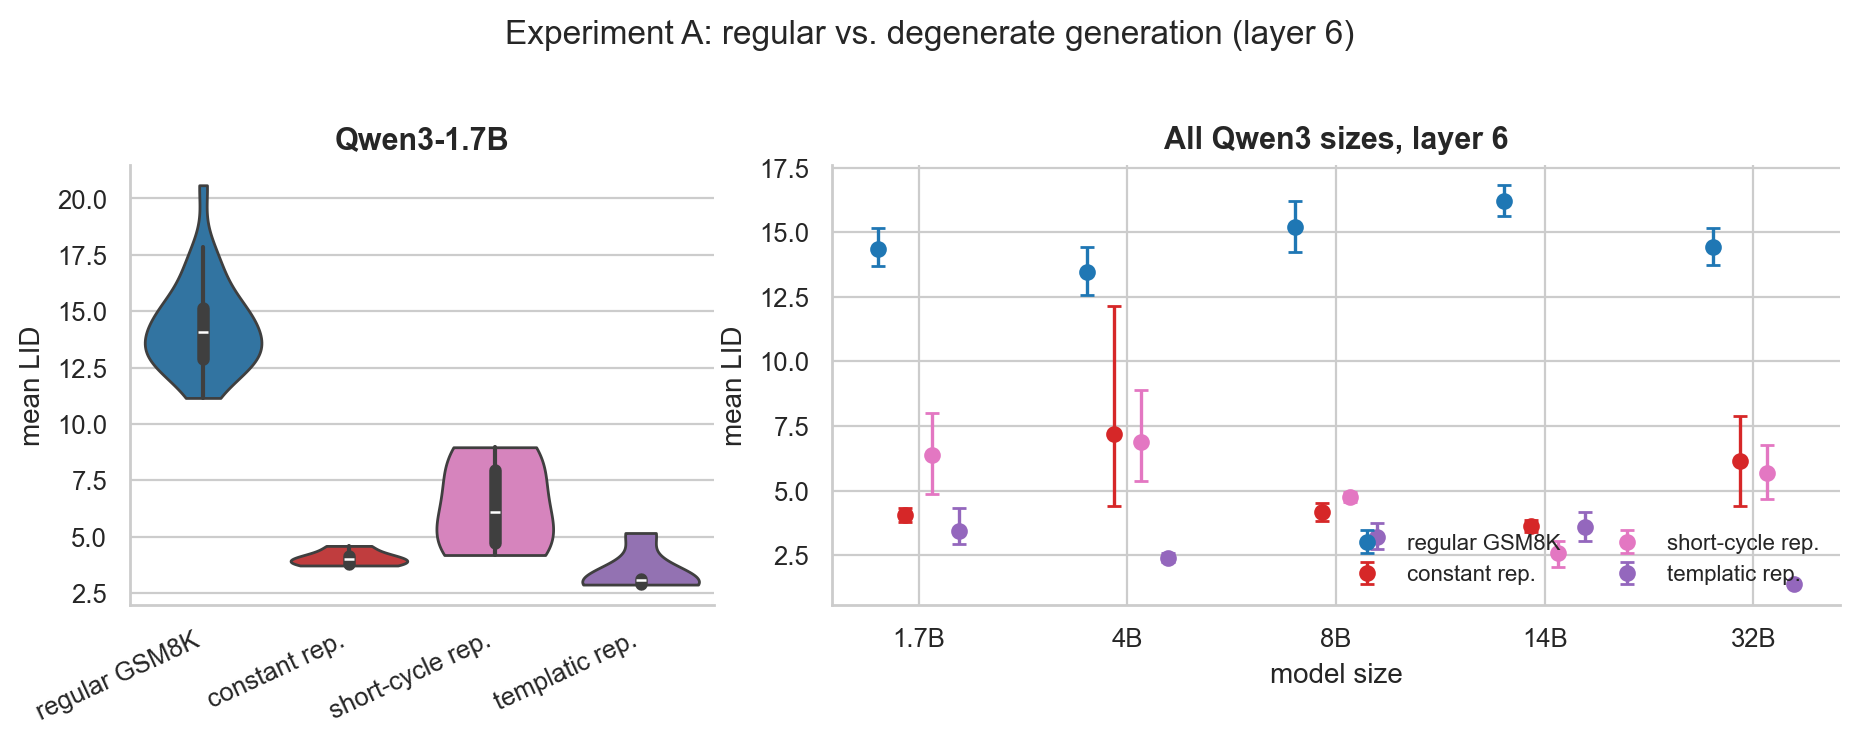
\includegraphics[width=0.95\linewidth]{Images/fig_exp_a_layer6.png}
    \caption{Experiment~A at layer~6. Conclusion as at layer~13: degenerate generation sits well below regular GSM8K at every model size.}
    \label{fig:app-exp-a-layer6}
\end{figure}

\begin{figure}[H]
    \centering
    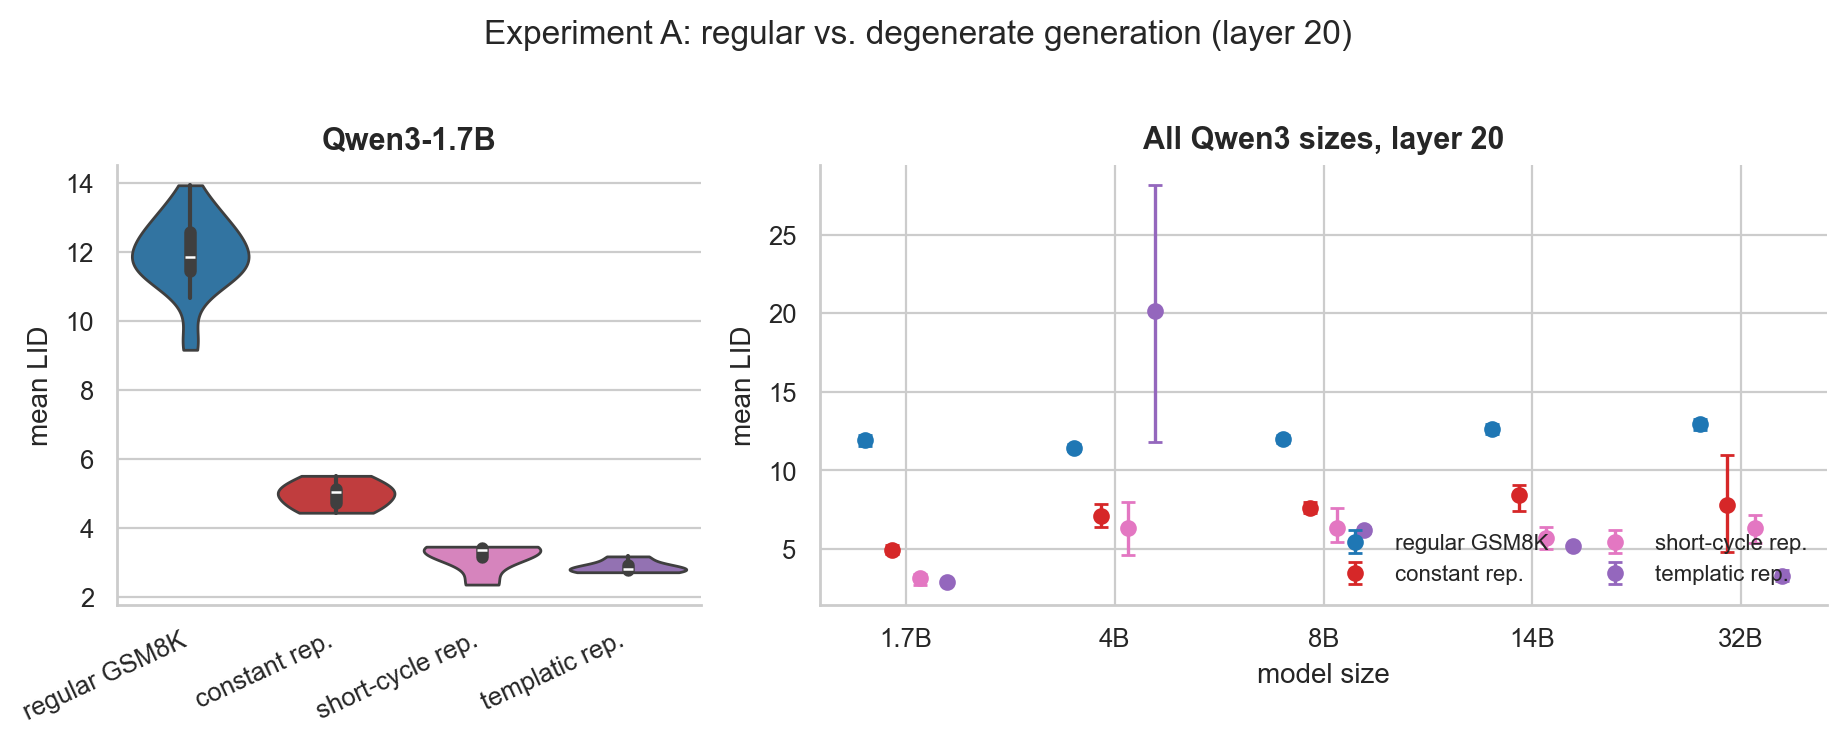
\includegraphics[width=0.95\linewidth]{Images/fig_exp_a_layer20.png}
    \caption{Experiment~A at layer~20. The separation between regular GSM8K and degenerate output is preserved; templatic repetition is again the lowest-LID family at most scales.}
    \label{fig:app-exp-a-layer20}
\end{figure}

\subsection{Experiment~B at layers 6 and 20}

\begin{figure}[H]
    \centering
    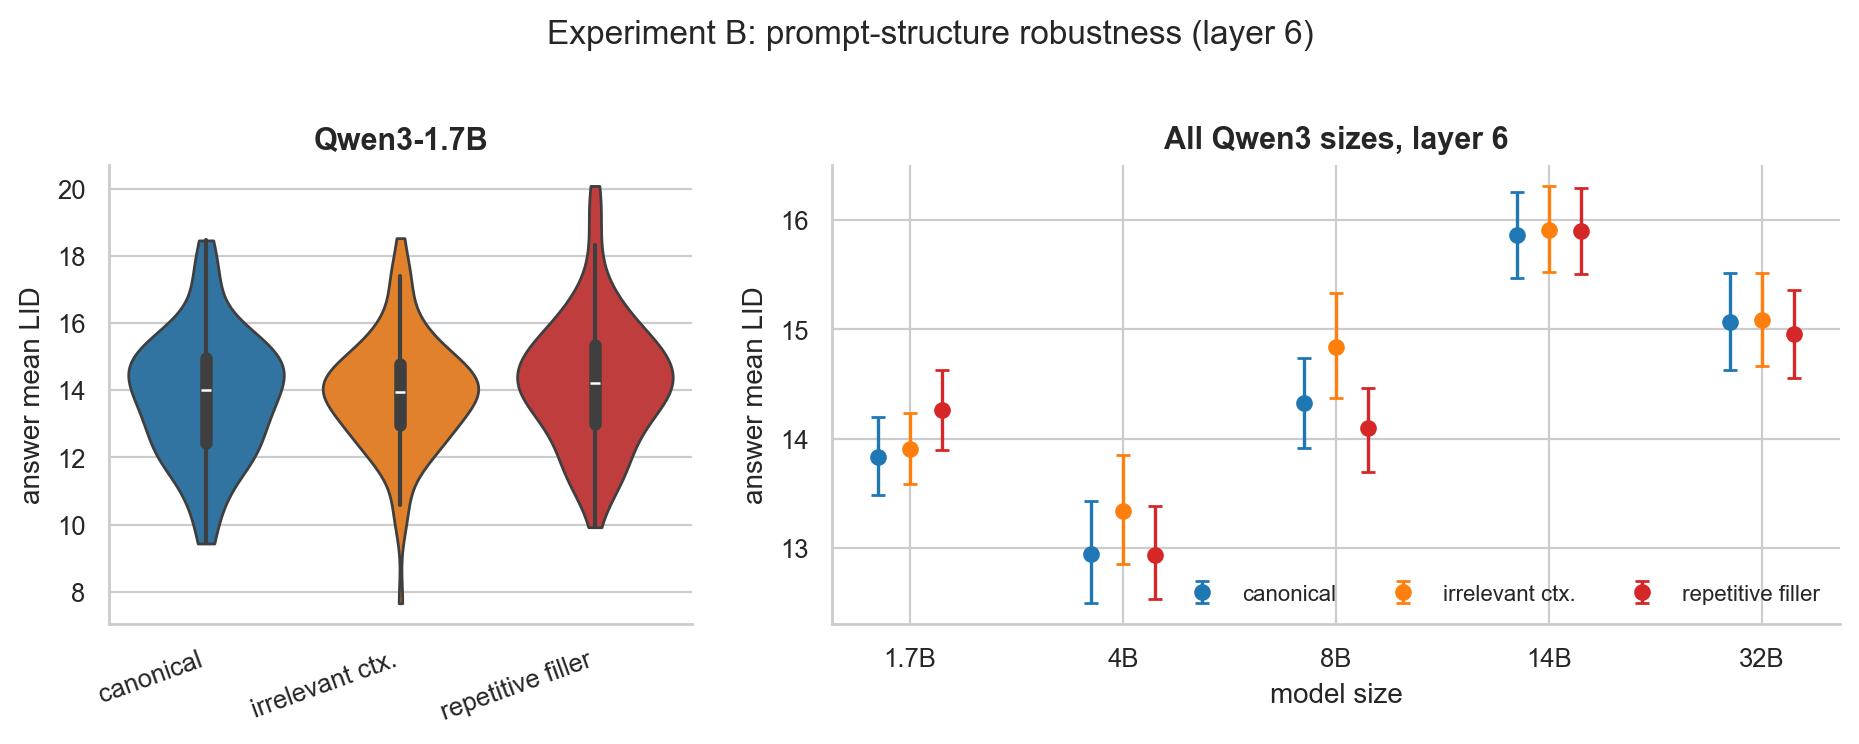
\includegraphics[width=0.95\linewidth]{Images/fig_exp_b_layer6.png}
    \caption{Experiment~B at layer~6. Canonical, irrelevant-context, and repetitive-filler answer-LID distributions are highly overlapping at every scale; the dominant axis of variation is model size, not prompt structure.}
    \label{fig:app-exp-b-layer6}
\end{figure}

\begin{figure}[H]
    \centering
    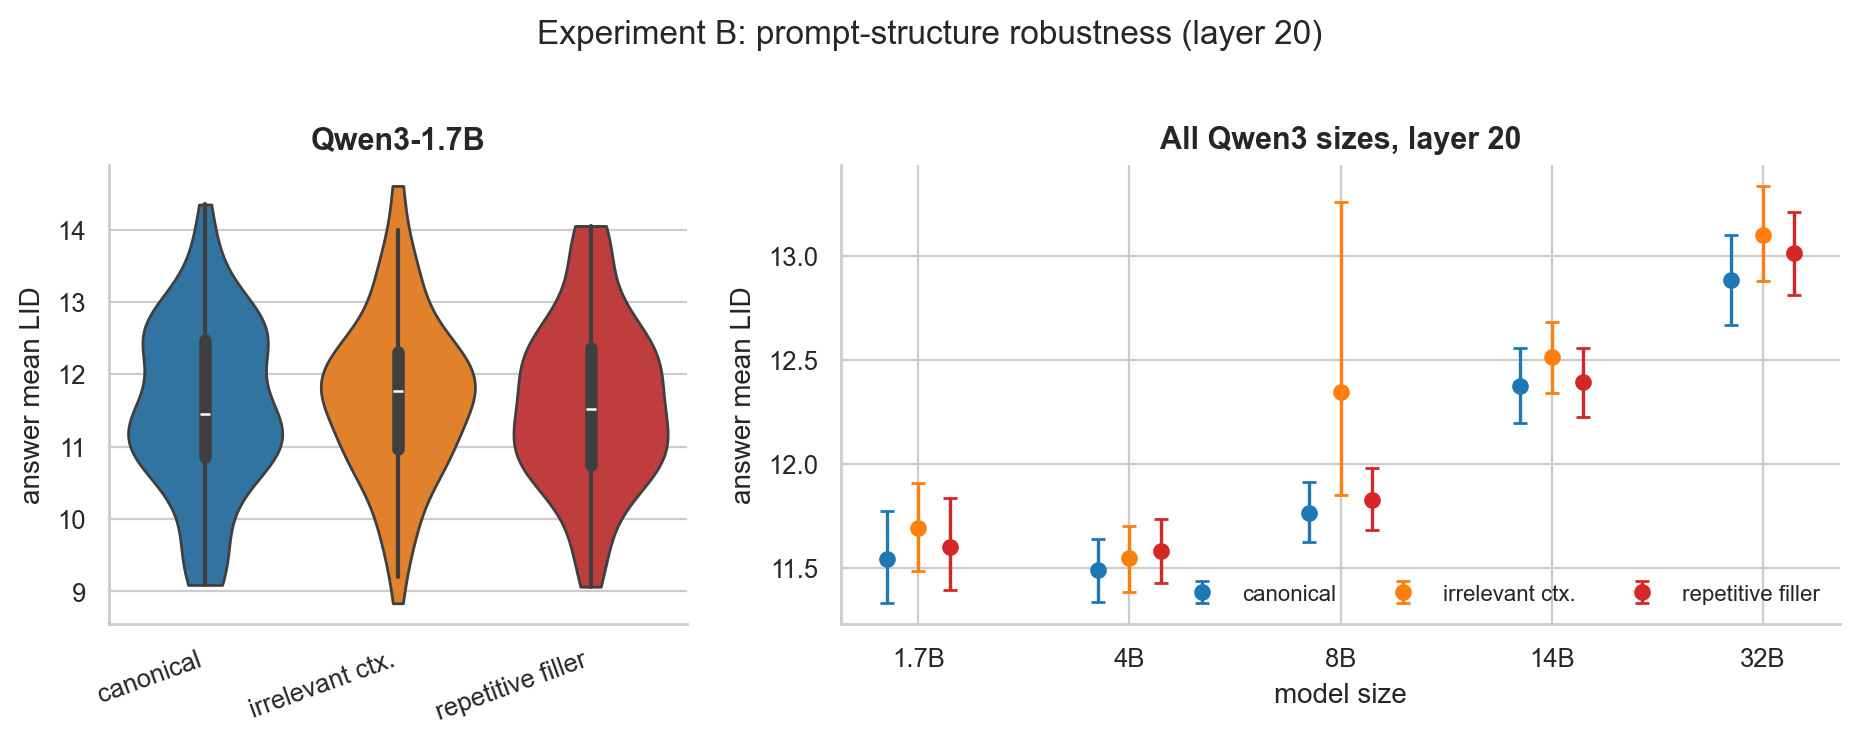
\includegraphics[width=0.95\linewidth]{Images/fig_exp_b_layer20.png}
    \caption{Experiment~B at layer~20. Prompt structure (including the deliberately repetitive filler prompt) does not move the answer-segment LID.}
    \label{fig:app-exp-b-layer20}
\end{figure}

\subsection{Experiment~C, C.1 (segment-level) at layers 6 and 20}

\begin{figure}[H]
    \centering
    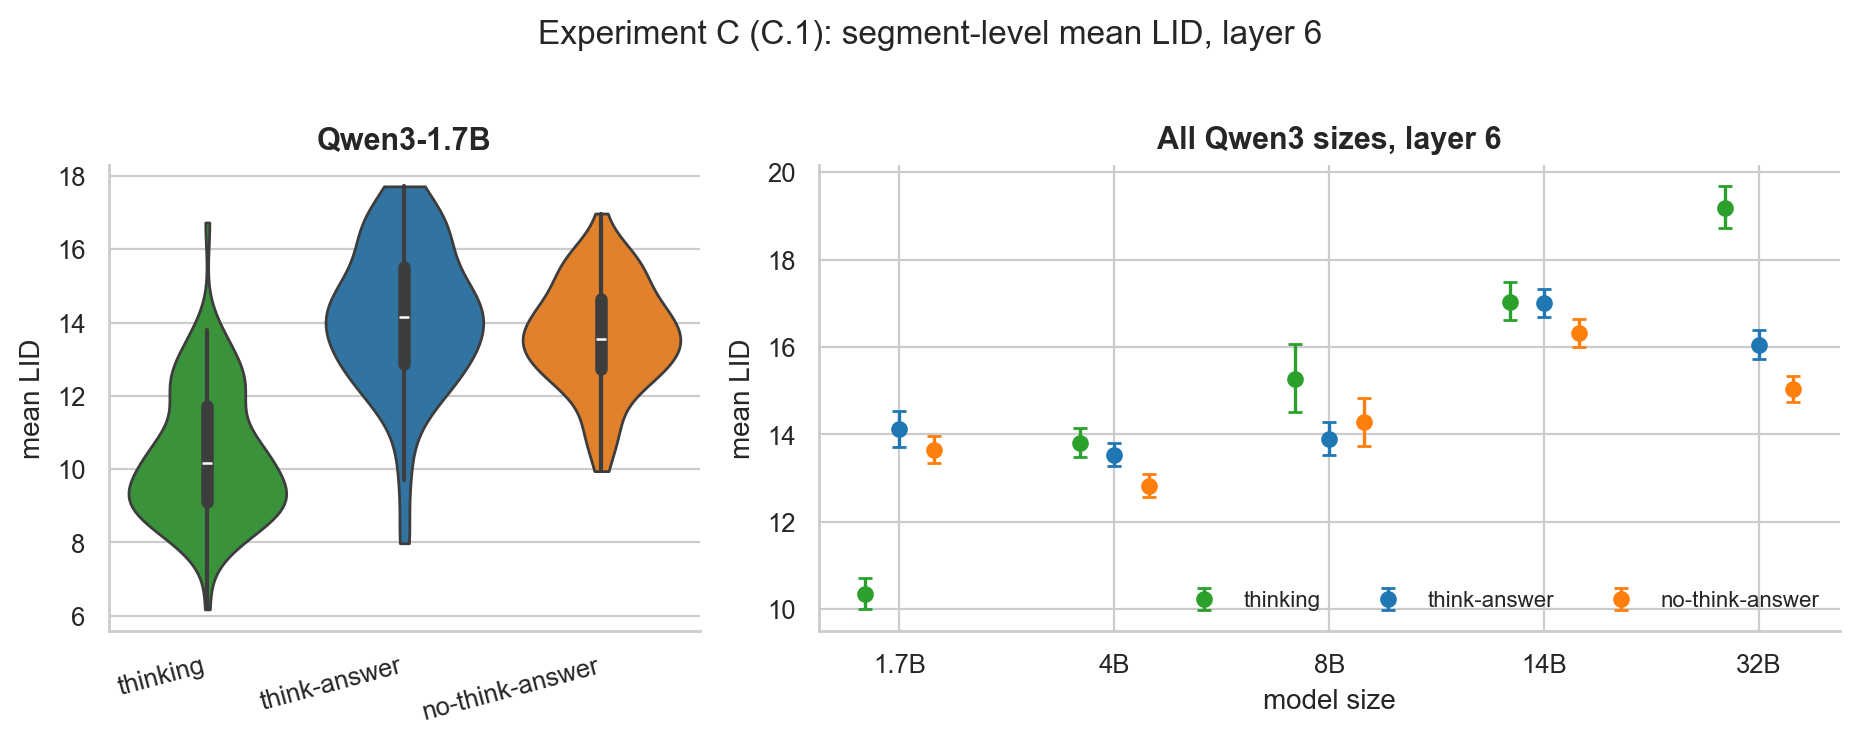
\includegraphics[width=0.95\linewidth]{Images/fig_exp_c_segments_layer6.png}
    \caption{Experiment~C, C.1 at layer~6. The ordering of the three segments inverts between Qwen3-1.7B (thinking is the lowest) and Qwen3-32B (thinking is the highest); see also \cref{tab:c1-wilcoxon-full}.}
    \label{fig:app-exp-c-layer6}
\end{figure}

\begin{figure}[H]
    \centering
    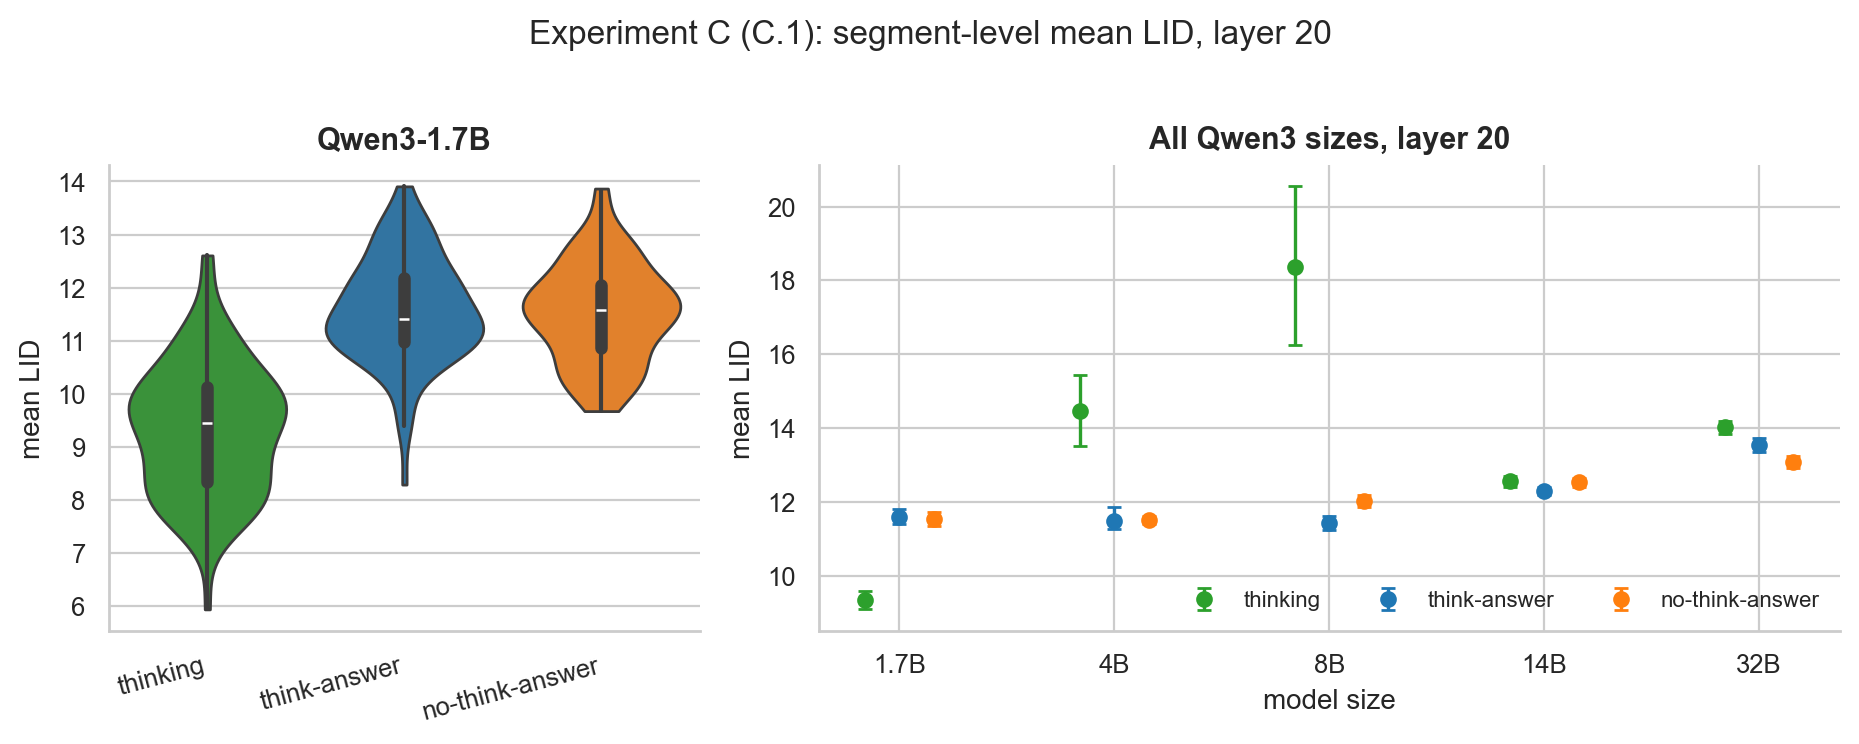
\includegraphics[width=0.95\linewidth]{Images/fig_exp_c_segments_layer20.png}
    \caption{Experiment~C, C.1 at layer~20. The segment ordering remains model-dependent, and is in particular different from layer~13.}
    \label{fig:app-exp-c-layer20}
\end{figure}

\subsection{Experiment~C, C.2 (correctness-stratified) at layers 6 and 20}

\begin{figure}[H]
    \centering
    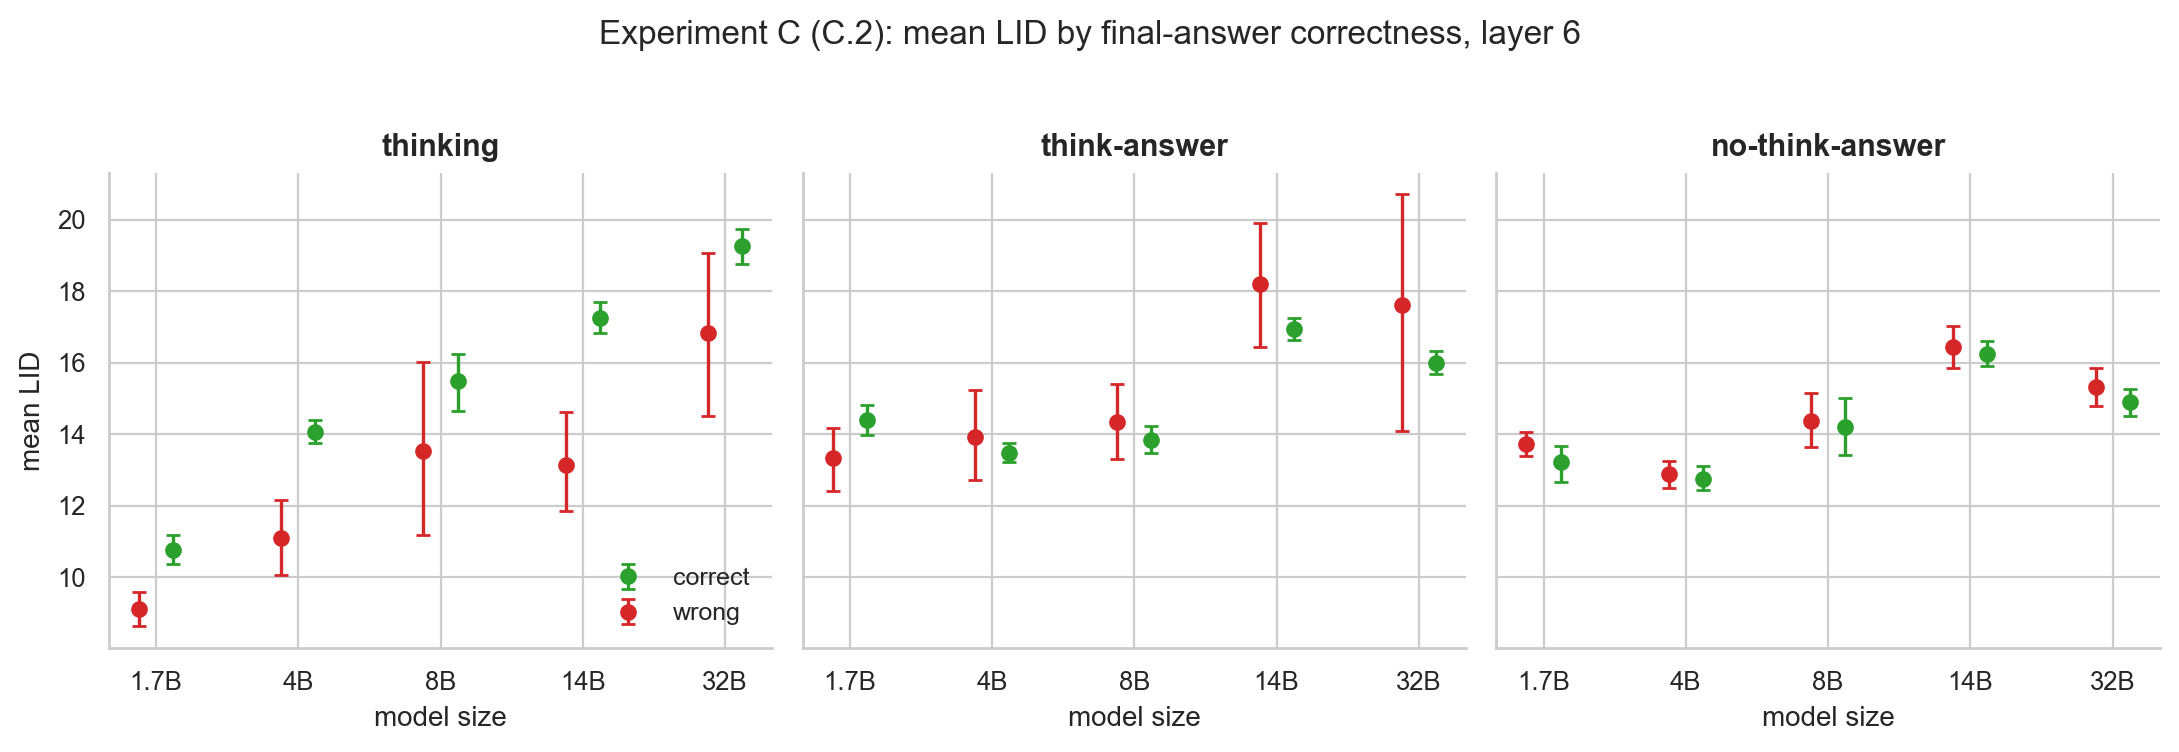
\includegraphics[width=0.95\linewidth]{Images/fig_exp_c_correctness_layer6.png}
    \caption{Experiment~C, C.2 at layer~6. The correctness gap in the thinking phase is positive at every model size (\cref{tab:c2-wilcoxon-full}); the gap in either answer phase is small with no consistent sign.}
    \label{fig:app-exp-c-corr-layer6}
\end{figure}

\begin{figure}[H]
    \centering
    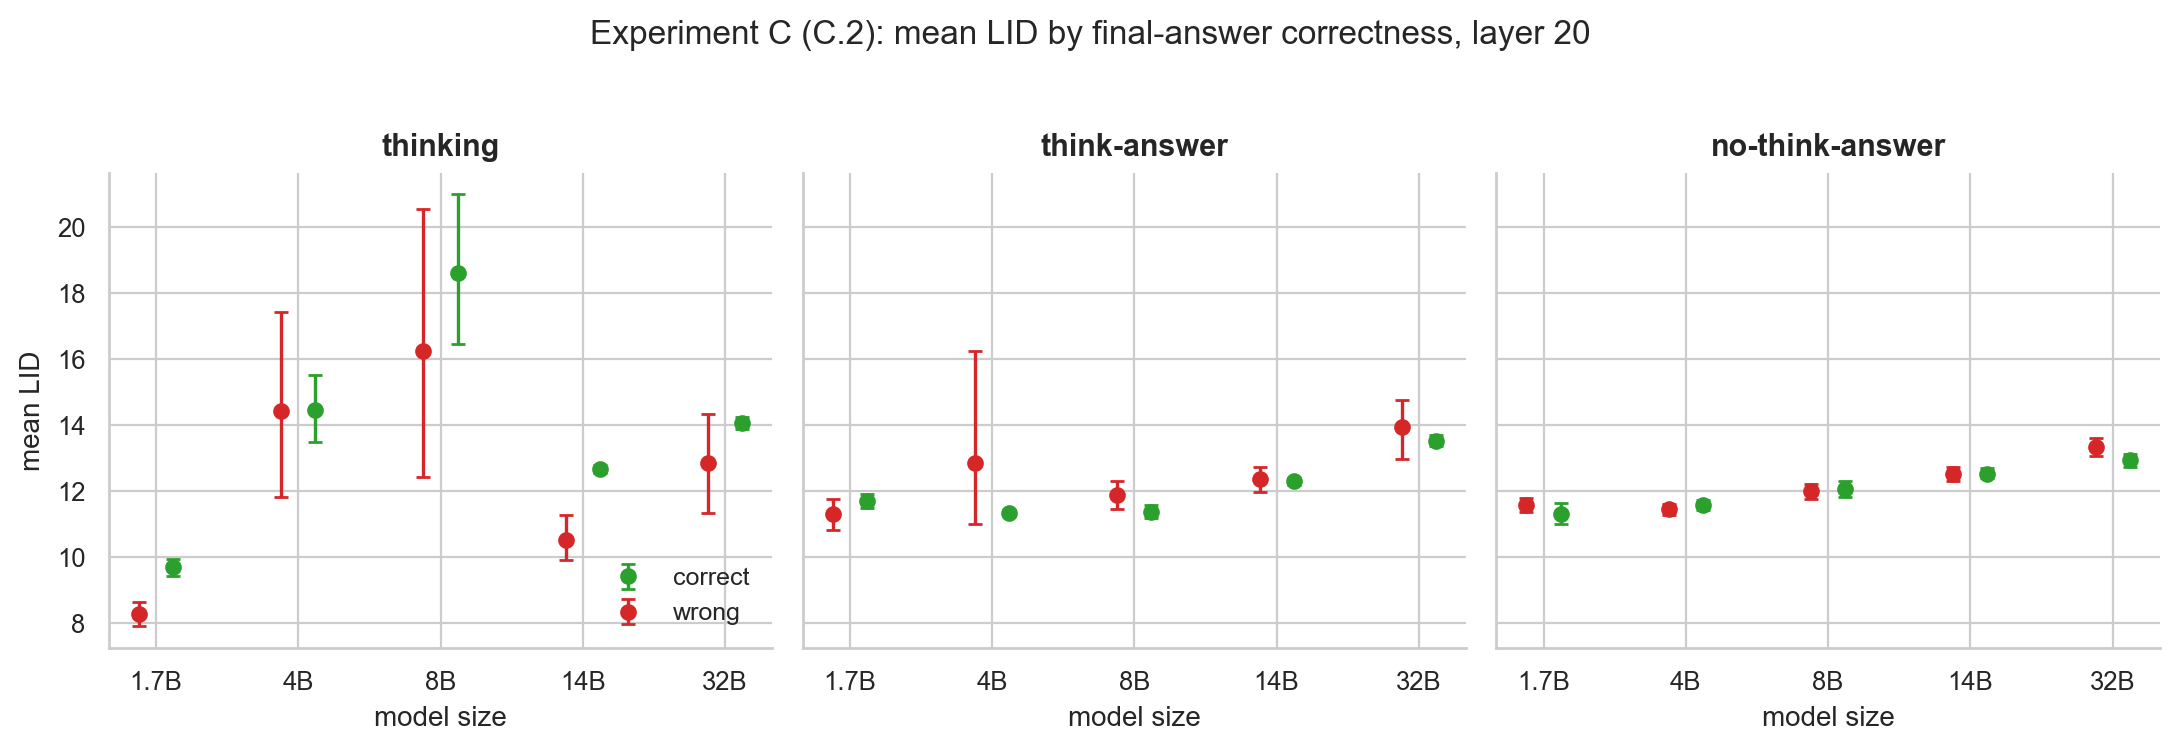
\includegraphics[width=0.95\linewidth]{Images/fig_exp_c_correctness_layer20.png}
    \caption{Experiment~C, C.2 at layer~20. The thinking-phase correctness gap stays positive at every model size; it is statistically strongest at layer~13 (\cref{tab:c2-wilcoxon-layer13}), but the sign is preserved here too.}
    \label{fig:app-exp-c-corr-layer20}
\end{figure}

\section{Per-Sample Token-Level Trajectory}
\label{app:token-trajectory}

\begin{figure}[H]
    \centering
    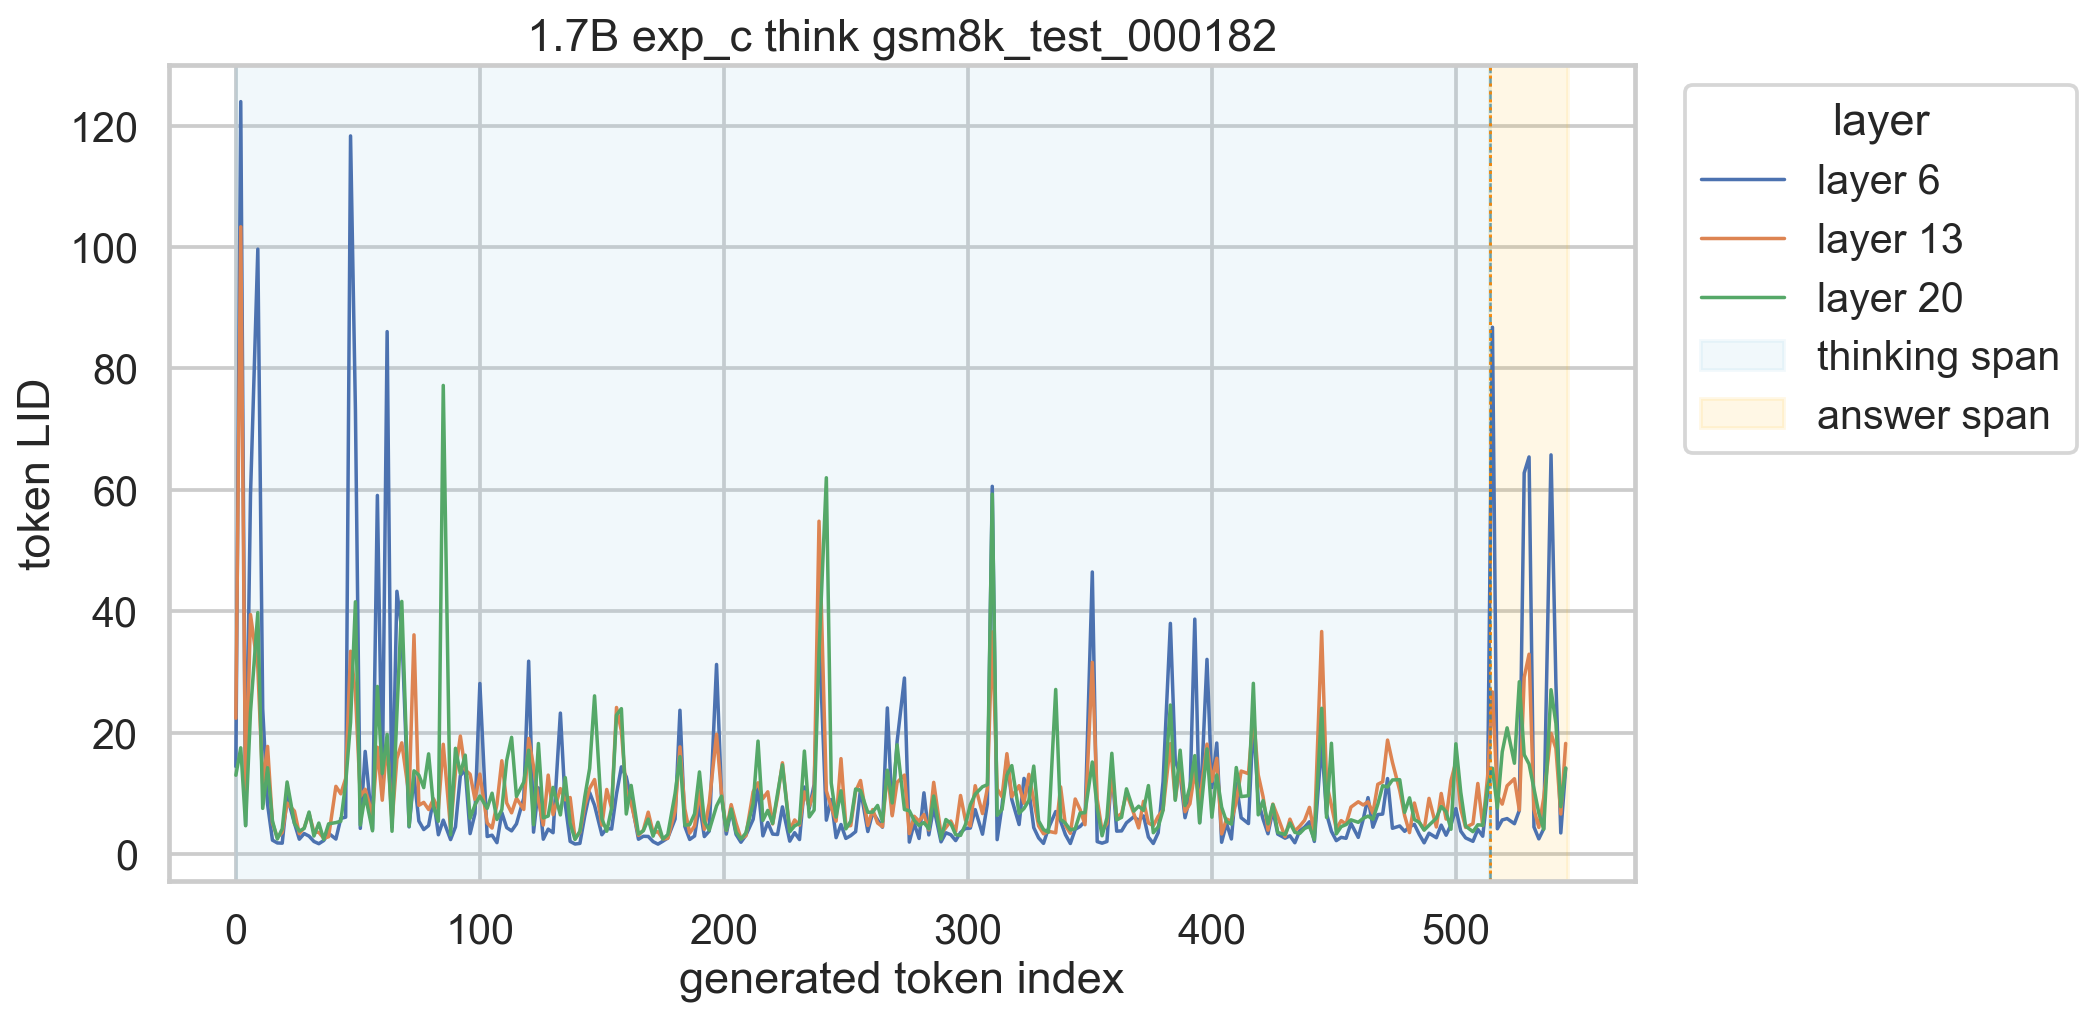
\includegraphics[width=0.7\linewidth]{Images/1.7B_think__gsm8k_test_000182.png}
    \caption{Token-level LID trajectory for a single Qwen3-1.7B think-mode GSM8K example, with the thinking and answer spans shaded. The token-level view shows that LID along a thinking trajectory is not flat, motivating the move from segment means (C.1) to within-segment, correctness-stratified analysis (C.2).}
    \label{fig:app-token-trajectory}
\end{figure}

\end{document}
